% Created 2024-03-25 Mon 12:31
% Intended LaTeX compiler: pdflatex
\documentclass[ee,thesis]{usuthesis}
\usepackage[utf8]{inputenc}
\usepackage[T1]{fontenc}
\usepackage{graphicx}
\usepackage{longtable}
\usepackage{wrapfig}
\usepackage{rotating}
\usepackage[normalem]{ulem}
\usepackage{amsmath}
\usepackage{amssymb}
\usepackage{capt-of}
\usepackage{hyperref}
\usepackage{amsmath}                        % Cool math
\usepackage{amsfonts}                       % Cool math fonts
\usepackage{amssymb}                        % Cool math fonts
\usepackage{booktabs}                       % Used for lines in table
\usepackage{lipsum}                         % Dummy filler text
\usepackage{graphicx}                       %
\usepackage{multicol}                       % Add capability to make columns
\usepackage{multirow}                       % Add capability to make rows
\usepackage{pgfgantt}                       % Add capability to create gantt charts
\usepackage{standalone}                     % Allow standalone documents
\usepackage{subfloat}                       % Subfigures
\usepackage{tabularx}                        % Add more contol to tables
\usepackage{listings}                       % Display code
\usepackage{doi}                            % Hyperlink DOI
\usepackage[ruled]{algorithm2e}                    % Algorithms
\usepackage{hyperref}                       %
\usepackage{subcaption}                     % Allow subfigures
\hypersetup{colorlinks=true, linkcolor=blue,
citecolor=blue,urlcolor=blue} % Use when compiling the digital copy
\usetikzlibrary{arrows.meta}                % Arrows for tikz
\renewcommand*{\chapterautorefname}{Chapter}
\renewcommand*{\sectionautorefname}{Section}
\renewcommand*{\subsectionautorefname}{Subsection}
\renewcommand*{\subsubsectionautorefname}{Subsubsection}
\renewcommand*{\paragraphautorefname}{Paragraph}
\renewcommand*{\algorithmautorefname}{Algorithm}
\newcommand{\definitionautorefname}{Definition}
\newcommand{\Or}{\textbf{ or }}
\renewcommand*{\And}{\textbf{ and }}
\newcolumntype{L}[1]{>{\hsize=#1\hsize\raggedright\arraybackslash}X}%
\newcommand\mycommfont[1]{\footnotesize\ttfamily\textcolor{gray}{#1}}
\newcommand{\T}{\mathcal{T}}                % To make it clear the difference
\newcommand{\Tau}{T}                        % between Tau and T
\newcommand{\AC}{AC(u, d, v, \eta)}            % Set the parameters for AC once
\newcommand{\PC}{PC(u, d, v)}               % Set the parameters for PC once
\newcommand{\ACi}{AC(u_i, d_i, q_i, \eta_i)}% Set the parameters for AC once
\newcommand{\PCi}{PC(u_i, d_i, q_i)}        % Set the parameters for PC once
\newcommand{\Not}{\textbf{not }}            % Custom `not' operator
\newcommand{\visit}{(b_i, a_i, e_i, u_i, d_i, q_i, \eta_i, \xi_i)}
\newcommand{\I}{\mathbb{I}}                 % Set of visit tuples
\newcommand{\C}{\mathbb{C}}                 % Charger availability information
\newcommand{\U}{\mathcal{U}}                % Uniform distribution
\newcommand{\W}{\mathcal{W}}                % Weighted distribution
\newcommand{\Sol}{\mathbb{S}}               % A shorthand for visit tuple
\newcommand{\M}{\mathbb{M}}                 % A shorthand for the metadata
\newcommand{\Hd}{\mathbb{H}}                % Set of discrete times
\newcommand{\Nu}{\mathcal{V}}               % Draw a nice Nu
\newcommand{\Iset}{I}                       % Set of visits 1-I
\newcommand{\Isetinit}{I_0}                 % Set of visits inital visits
\newcommand{\Isetfinal}{I_f}                % Set of visits final visits
\newcommand{\Bset}{B}                       % Set of visits 1-B
\newcommand{\Qset}{Q}                       % Set of visits 1-Q
\newcommand{\Jset}{J}                       % Set of visits 1-J
\newcommand{\Jsetq}{\mathbb{J}}             % Set of visits 1-J for queue active times
\newcommand{\Hset}{H}                       % Set of visits 1-H
%%-------------------------------------------------------------------------------
% Experiment parameters
\newcommand{\A}{35 }                                                            % Number of buses
\newcommand{\N}{338 }                                                           % Number of visits
\newcommand{\Cgain}{5000}                                                       % Gain applied to penalty method
\newcommand{\acharge}{0.9}                                                      % BOD charge percentage
\newcommand{\bcharge}{0.7 }                                                     % EOD charge percentage
\newcommand{\mincharge}{25\% }                                                  % Min visit charge percent
\newcommand{\minchargeD}{0.25 }                                                 % Min visit charge decimal
\newcommand{\maxcharge}{100\% }                                                 % Max visit charge percent
\newcommand{\batsize}{388 }                                                     % Battery capacity
\newcommand{\fast}{15 }                                                         % Number of fast chargers
\newcommand{\slow}{15 }                                                         % Number of slow chargers
\newcommand{\fasts}{911 }                                                       % Speed of fast charger
\newcommand{\slows}{30 }                                                        % Speed of slow charger
\newcommand{\contvars}{7,511 }
\newcommand{\intvars}{328,282 }
\newcommand{\localcnt}{500 }                                                    % Number of local search iterations
\newcommand{\tempinit}{9000 }                                                   % Initial temperature
\newcommand{\tempcnt}{9101 }                                                    % Number of steps in temperature
\newcommand{\quicklocal}{0.25 }                                                % Time to finish local quick
\newcommand{\heuristiclocal}{0.4 }                                             % Time to finish local heuristic
%%-------------------------------------------------------------------------------
%% Solve output
%% Solve output
\newcommand{\timeran}{4.2 }                                                    % Time ran for MILP [s]
% The Committee
\majorprof{Dr. Greg Droge, Ph.D.}
\firstreader{Dr. Jacob Gunther, Ph.D.}
\secondreader{Dr. Burak Sarsilmaz, Ph.D.}

% Graduate Dean
\graddean{ D. Richard Cutler, Ph.D.}
\deantitle{ Vice Provost of Graduate Studies}

% Degree Information
\degree{Master of Science}
\month{Dec}
\gradyear{2024}
\newtheorem{definition}{Definition}[section]
\author{Alexander Brown}
\date{}
\title{The Simulated Annealing Fully Fuzzy Position Allocation Problem Utilizing Mixed Integer Linear Programming Constraints with Non-Linear Battery Dynamics}
\hypersetup{
 pdfauthor={Alexander Brown},
 pdftitle={The Simulated Annealing Fully Fuzzy Position Allocation Problem Utilizing Mixed Integer Linear Programming Constraints with Non-Linear Battery Dynamics},
 pdfkeywords={},
 pdfsubject={},
 pdfcreator={Emacs 29.3 (Org mode 9.6.15)}, 
 pdflang={English}}
\begin{document}

\let\ref\autoref                            % Redifine `\ref` as `\autoref` because lazy
\SetCommentSty{mycommfont}                  % Set the comment color

\preliminaries   % set frontmatter style

\maketitle

\tableofcontents
\listoftables
\listoffigures

\body  % set main body style

\chapter{INTRODUCTION}
\label{sec:introduction}
Public transportation systems are crucial in any urban area; however, the increased awareness and concern of
environmental impacts of petroleum based public transportation has driven an effort to reduce the pollutant footprint
\cite{de-2014-simul-elect,xylia-2018-role-charg,guida-2017-zeeus-repor-europ,li-2016-batter-elect}. Particularly,
the electrification of public bus transportation via battery power, i.e., battery electric buses (BEBs), has received
significant attention \cite{li-2016-batter-elect}. Although the technology provides benefits beyond reduction in
emissions, such as lower driving costs, lower maintenance costs, and reduced vehicle noise, battery powered systems
introduce new challenges such as larger upfront costs, and potentially several hours long ``refueling'' periods
\cite{xylia-2018-role-charg,li-2016-batter-elect}. Furthermore, the problem is exacerbated by the constraints of the
transit schedule to which the fleet must adhere, the limited amount of chargers available, and the adverse affects in
the health of the battery due to fast charging \cite{lutsey-2019-updat-elect}.

BEBs have been in service for many major markets, North America, Europe, and China, for more than a decade with expected
growth in the near future \cite{deng-2021-survey-elect}. The Asia Pacific market is forecasted to dominate the sales
and some major companies of the industry have also begun to enter the global market such as Volvo, BYD, and Proterra by
2025 \cite{deng-2021-survey-elect}. Much focus has been placed on the engineering of individual BEBs such as battery
type, brake regenerative charging, optimal battery charging, and battery degradation \cite{chen-2008-desig-grey,abdollahi-2016-optim-batter,kuhne-2010-elect,deng-2021-survey-elect}. The interest of route scheduling, charging
fleets, and optimizing the infrastructure are problems of more recent interest and are therefore timely and increasingly
relevant problems as EV/BEBs become more commonplace \cite{hoke-2014-accoun-lithium,sebastiani-2016-evaluat-elect,wei-2018-optim-spatio}.

The literature shows an interest in solving the problem of assigning BEBs to charging queues or optimizing their
infrastructure \cite{wei-2018-optim-spatio,sebastiani-2016-evaluat-elect,hoke-2014-accoun-lithium,wang-2017-elect-vehic}. In fact, many works attempt to solve both problems simultanously
barring some simplification whether it be only allowing chargers of a single type
\cite{he-2020-optim-charg,tang-2019-robus-sched}. If multiple chargers are used, then one of each type is assigned at
each location. Others have also assumed that a BEB shall recieve full charge upon each arrival
\cite{wei-2018-optim-spatio,wang-2017-elect-vehic,zhou-2020-bi-objec,wang-2017-optim-rechar}. Some works on the
stochastic effects of energy consumption while on route for a BEB as well as trip times \cite{zhou-2020-collab-optim,bie-2021-optim-elect}. One other source, as far as the reseach for this work has shown, describes a method of producing
a BEB charge schedule wih a high fidelity while accounting for multiple charger times as well as being able to minimize
over the total charger count \cite{whitaker-2023-a-network}.

The work described in this proposal is similar to the work in \cite{whitaker-2023-a-network}; however provides an
alternate method of modeling the problem in what is known as the Position Allocation Problem (PAP). The PAP is modeled
after the Berth Allocation Problem (BAP), which was designed to optimally schedule cargo vessels to be berthed and
serviced \cite{buhrkal-2011-model-discr,imai-2001-dynam-berth,frojan-2015-contin-berth}. The PAP utilizes this
notion to develop a model of assigning EVs to queue in ordered to be charged \cite{qarebagh-2019-optim-sched}.

Because of the PAP's extremely close modeling methods to the BAP, literature from the BAP can (and will) provide support
for the development of the PAP in this work. The BAP has been studied in literature since the 1990s and provides a depth
of work to derive from \cite{rodrigues-2022-berth}. The work to be introduced promises much potential for further
research and development in regard to scheduling BEBs. What follows is a proposal for a Simulated Annealing (SA)
implementation and extension of the PAP utilizing Mixed Integer Linear Programming (MILP) constraints with non-linear
battery dynamics.

In the next section, a review of relevant literature of BEBs is introduced and discussed. Background and a problem
statement will be elaborated further to provide context and a required basis of understanding prior to discussing the
objectives and approaches in \ref{sec:objectives} and \#sec:approach]], respectively. The BEB queue scheduling problem discussed
throughout this section is of particular interest at this time in the BEB industry and requires more attention. The
research proposed directly approaches this problem by improving upon existing implementations to provide a robust and
accurate solution. In the subsequent sections the objectives will be introduced in \ref{sec:objectives} and the approach for
each objective will be discussed in \#sec:approach]].

\section{OBJECTIVES}
\label{sec:objectives}
The field of BEB research provides exciting many avenues and is continuing to gain traction in industry as BEBs replace
their gasoline counterparts. This work will introduce a novel approach to BEB scheduling that minimizes monetary costs
for the user, provides a robust solution, and includes an accurate dynamic battery model. The PAP provides a solid
foundation from which this work derived. However, the PAP does not perfectly encapsulate the problem and thus needs some
modifications to accommodate the BEB model. The PAP does not account for the revisits of a BEB and therefore the
State-Of-Charge (SOC) cannot be tracked. The model does not account for multiple charger types, and in fact models the
charger as a single continuous bar. These accommodations must be accounted for and are included in the objectives for
the proposed BEB charging plan below.

\begin{itemize}
\item \textbf{Objective 1}: Mathematically model the PAP to optimally assign BEBs to queues with unknown charging times to allow consideration of consumption cost and battery health

\begin{itemize}
\item \textbf{Task 1.1}: Modify PAP to enable multiple visits by a BEB with variable charger duration per visit.

\item \textbf{Task 1.2}: Incorporate heterogeneous charger capabilities into the PAP to model slow and fast charging, minimize
and total charger count. Slow charging will be incentivized for battery health and consumption cost.
\end{itemize}

\item \textbf{Objective 2}: Mathematically model non-linear battery dynamics to increase the accuracy of the SOC estimate

\begin{itemize}
\item \textbf{Task 2.1}: Incorporate non-linear battery dynamics into the model
\end{itemize}
\end{itemize}
\chapter{BACKGROUND AND RELATED WORK}
\label{sec:background-and-related-work}
The BEB queue scheduling problem is one that has been of increasing interest and relevancy in the EV/BEB industry. It is
thus important to address the state of the art by introducing relevant problems in BEB queue scheduling, which will be
addressed first. A detailed problem description shall then be presented to provide a basis of understanding of the
proposition. Relevant introductory theory will be presented throughout.

\section{State Of The Art of Battery Electric Bus Charging}
\label{sec:state-of-the-art}
Two of the main problems that have been of recent interest are solving the problems of route scheduling and charging
fleets as well as determining the infrastructure upon which they rely. In fact, the prospect of solving both problems
simultaneously has received much attention \cite{wei-2018-optim-spatio,sebastiani-2016-evaluat-elect,hoke-2014-accoun-lithium,wang-2017-elect-vehic}. These problems vary by including assignment of buses to routes
\cite{rinaldi-2020-mixed-fleet,zhou-2020-collab-optim,tang-2019-robus-sched,li-2014-trans-bus}, determining
whether a set of existing combustion based buses should be replaced with BEBs \cite{zhou-2020-bi-objec,duan-2021-refor-mixed,rinaldi-2020-mixed-fleet,zhou-2020-collab-optim}, and accounting for uncertainties
\cite{bie-2021-optim-elect,duan-2021-refor-mixed,tang-2019-robus-sched,ursavas-2016-optim-polic}. These problems
add additional complexities that warrant simplifications due to computational complexities.

Several simplifications are made throughout the literature to make these problems computationally feasible. These
simplifications to the charge scheduling model include utilizing only fast chargers while planning
\cite{wei-2018-optim-spatio,sebastiani-2016-evaluat-elect,wang-2017-optim-rechar,zhou-2020-bi-objec,yang-2018-charg-sched,wang-2017-elect-vehic,qin-2016-numer-analy,liu-2020-batter-elect}. If slow chargers are used,
they are only deployed at the one location with fast chargers being deployed elsewhere
\cite{he-2020-optim-charg,tang-2019-robus-sched}. Some approaches also simplify by assuming a full charge is always
achieved \cite{wei-2018-optim-spatio,wang-2017-elect-vehic,zhou-2020-bi-objec,wang-2017-optim-rechar}.

In some works, it was assumed that the charge received is proportional to the time spent on the charger
\cite{liu-2020-batter-elect,yang-2018-charg-sched}. While the linear battery dynamics is a valid assumption when the
battery SOC is below 80\% \cite{liu-2020-batter-elect}, non-linear battery dynamics can be implemented to more accurately
model the charge curve. A common way to model the non-linear battery dynamics is utilizing Constant Voltage (CV),
Constant Current (CC), and Constant Current Constant Voltage (CCCV) \cite{abdollahi-2016-optim-batter,chen-2008-desig-grey}. It has also been suggested that the dynamics can be modeled as a piecewise function containing a
linear and non-linear component from which a piecewise function approach may be taken for the CV and CC components
\cite{zhang-2021-optim-elect,abdollahi-2016-optim-batter}. Others have modeled the battery dynamics as a discrete
first order dynamics model \cite{whitaker-2023-a-network}. The first-order differential system, when provided a step
input, approximates the non-linear relationship between time and the current SOC \cite{whitaker-2023-a-network}.

Works concerning charge planning often use a version of the vehicle scheduling problem \cite{tang-2019-robus-sched,li-2014-trans-bus,he-2020-optim-charg}. Variants of this problem address infrastructure as well as determining
existing buses that should be replaced by a BEB \cite{zhou-2020-bi-objec,duan-2021-refor-mixed,rinaldi-2020-mixed-fleet,zhou-2020-collab-optim}. Other works introduce a directed graph approach to model the flow
of BEBs \cite{whitaker-2023-a-network,liu-2020-batter-elect}, where this concept was expanded to simultaneously
accounting for multiple charger types, partial charging, non-linear battery charge profiles
\cite{whitaker-2023-a-network}. The directed graph approach provides an easy method of modeling the scheduling by
discretizing the time horizon to \(n_Q\) sets of nodes. The nodes represent the chargers availability and can have a
maximum of one bus at a time. The buses can flow into a node to be charged and then later can exit allowing a new bus to
enter. Another method similar to the directed graph that fits the modeling of the BEB charging scenario is the PAP
\cite{qarebagh-2019-optim-sched}. The PAP is derived from the BAP which takes an input of vessel arrival times and
outputs the selection of the berthing quay. The PAP utilizes this model and redefines its inputs to EV arrival times and
outputs queues for the EVs to be charged. While the visits remain as discrete events, the time that the BEB is on the
charger is modeled in continuous time similar to \cite{frojan-2015-contin-berth,qarebagh-2019-optim-sched,zhou-2020-collab-optim}. Due to the close relationship between the BAP and PAP, BAP
literature may be used for the PAP. The literature shows methods of handling multiple quays (sets of chargers) to handle
general berthing scenarios \cite{frojan-2015-contin-berth,dai-2008-suppl-chain-analy}. Heuristic procedures for
quicker solve times have also been introduced \cite{imai-2001-dynam-berth}. Methods of defining static (full time
horizon) and dynamic (rolling-time horizon) models have been created for daily and real-time solutions, respectively,
and even fuzzy set theory has been applied to allow for more flexible schedules \cite{bello-2019-fuzzy-activ}.

\section{Problem Description}
\label{sec:problem-description}
The intent of the proposed work is to build upon the Position Allocation Problem \cite{qarebagh-2019-optim-sched}, a
modification of the well studied Berth Allocation Problem (BAP), as a means to schedule the charging of electric
vehicles \cite{buhrkal-2011-model-discr,frojan-2015-contin-berth,imai-2001-dynam-berth}. The PAP's goal is that of
allocating space for incoming BEBs to be queued and charged as depicted in \autoref{subfig:papexample}. The BEBs are
assumed to be on schedules that are defined in advance. That is, the times the BEBs are on their respective routes and
the time they are at the station are known. The BEBs' initial charges are assumed to be known, the discharges are
estimated by calculating an average bus speed, the time on route, and an average amount of energy consumed per mile, and
a specified final charge must be met for each BEB. An example of a standard PAP/BAP solution (their visual
representations are interchangeable) is visualized in \autoref{fig:bap}, note that the figure utilized BAP terminology.
The x and y-axis represent time and queuing space, respectively. The figure discretizes the queuing space, but it may be
continuous if desired as previously stated. The shaded rectangles' widths represent their respective allocated charge
times, and their heights represent the physical space taken by each EV.

\begin{subfigures}
    %%~~~~~~~~~~~~~~~~~~~~~~~~~~~~~~~~~~~~~~~~~~~~~~~~~~~~~~~~~~~~~~~~~~~~~~~~~~~~
    % BAP
    \begin{figure}[htpb]
    \centering
        \includestandalone{sup-doc/milp-pap-paper-frontiers/img/bap}
        \caption{Example of berth allocation. Vessels are docked in berth locations (horizontal) and are queued over
          time (vertical). The vertical arrow represents the movement direction of queued vessels and the horizontal
          arrow represents the direction of departure.}
        \label{subfig:bapexample}
    \end{figure}
    \hfill

    %%~~~~~~~~~~~~~~~~~~~~~~~~~~~~~~~~~~~~~~~~~~~~~~~~~~~~~~~~~~~~~~~~~~~~~~~~~~~~
    % PAP
    \begin{figure}[htpb]
    \centering
        \includestandalone{sup-doc/milp-pap-paper-frontiers/img/pap}
        \caption{Example of position allocation. Vehicles are placed in queues to be charged and move in the direction
          indicated by the arrow.}
        \label{subfig:papexample}
    \end{figure}
\end{subfigures}

Now that the problem has been defined conceptually, the problem shall be defined in more mathematical terms.
supplied from any single charger given a set of chargers at the station. Let the term ``arrival'' describe the time at
which a BEB reaches the station. Furthermore, let the term ``visit'' denote a BEB having arrived, awaited its
predetermined time (whether it has received a charge or not), and departed from the station. Each BEB may have multiple
visits to the station throughout their working day. This paper describes a method to optimize the assignment of each
visit to a charger given a schedule for a fleet of BEBs that follow the behavior described above. The model presented in
this work optimizes over peak power usage and energy consumption, as well as attempts to optimize the amount of chargers
utilized.

Consider a fleet of \(n_B\) BEBs that collectively visit a station \(n_V\) times. At said station, let there exist a pool of
\(n_Q\) charging queues from which a visiting BEB may be assigned. Let \(\mathbb{Z}\) define the set of integers. The pool of queues
from which a BEB may be placed is \(\Qset \subset \mathbb{Z}\) is defined by letting the first \(n_B\) queues be denoted as idle queues
followed by slow and then fast chargers. The term idle queues is meant to signify queues that provide no charge to the
BEB. The next \(n_Q\) queues are chargers ordered from slow to fast. Furthermore, let the set of arrivals be denoted as
\(\Iset = \{ 1, ... n_V \} \subset \mathbb{Z}\). Each BEB is provided an identification number in the set \(B = \{ 1, ..., n_B \} \subset \mathbb{Z}\).
Each visit can be represented by the tuple: \(\visit\), in which the elements within the tuple denote the visit index, \(i
\in I\), BEB identification number, \(b \in B\), arrival time to the station, \(a \in \mathbb{R}\), departure time from the station, \(e \in
\mathbb{R}\), time at which the BEB begins charging, \(u \in \mathbb{R}\), time at which the BEB ends charging, \(d \in \mathbb{R}\), the charger queue for
the BEB to be placed into, \(q \in Q\), the SOC upon arrival, \(\eta \in \mathbb{R}\), and the index of the next visit for the currently
visiting BEB, \(\xi \in I \cup \varnothing\). The null element, \(\varnothing\), is used to specify when a BEB has no future
visits. Let the ordered set of visits be denoted as \(\I\) where the \(i^{\text{th}}\) visit is denoted is \(\I_i\).
Furthermore, let a particular item from the tuple for visit \(i\) to be written as \(\cdot_i\). For example, the arrival time
for visit \(i\) is written as \(a_i\).

At each visit, the associated BEB is placed into a single queue corresponding to a particular charger. The charger is
assumed to be either an idle queue, slow charger, or fast charger. A BEB is only allowed to be assigned to one queue per
visit; however, there may be multiple BEBs charging simultaneously across different queues. The amount of time the BEB
is allowed to charge during visit \(i\) is dictated by the scheduled arrival time and required departure time, \([a_i,
e_i]\). Partial charging is allowed; however, the SOC may not exceed the BEB battery capacity and the SOC must stay above
0\%. The battery dynamics in this work is modeled as linear, which remains accurate up to about an SOC of 80\% charge
\cite{liu-2020-batter-elect}. Note that charging beyond the 80\% SOC threshold is undesirable due to batter health
concerns.

Each BEB arrival, except for the last arrival for each BEB, has a paired ``route'' that the BEB must perform after the
visit. This route, as one would expect, causes the BEB to discharge by some certain amount. Each bus is assumed to have
a fixed discharge. Let the discharge of the route for visit \(i\) be denoted as \(\Delta_i \in \mathbb{R}\). Each bus has a desired minimum
battery percentage, \(\nu_b \in [0, 1]\).

\begin{figure}[ht!]
  \centering
  \scalebox{0.5}{
  \centerline{
    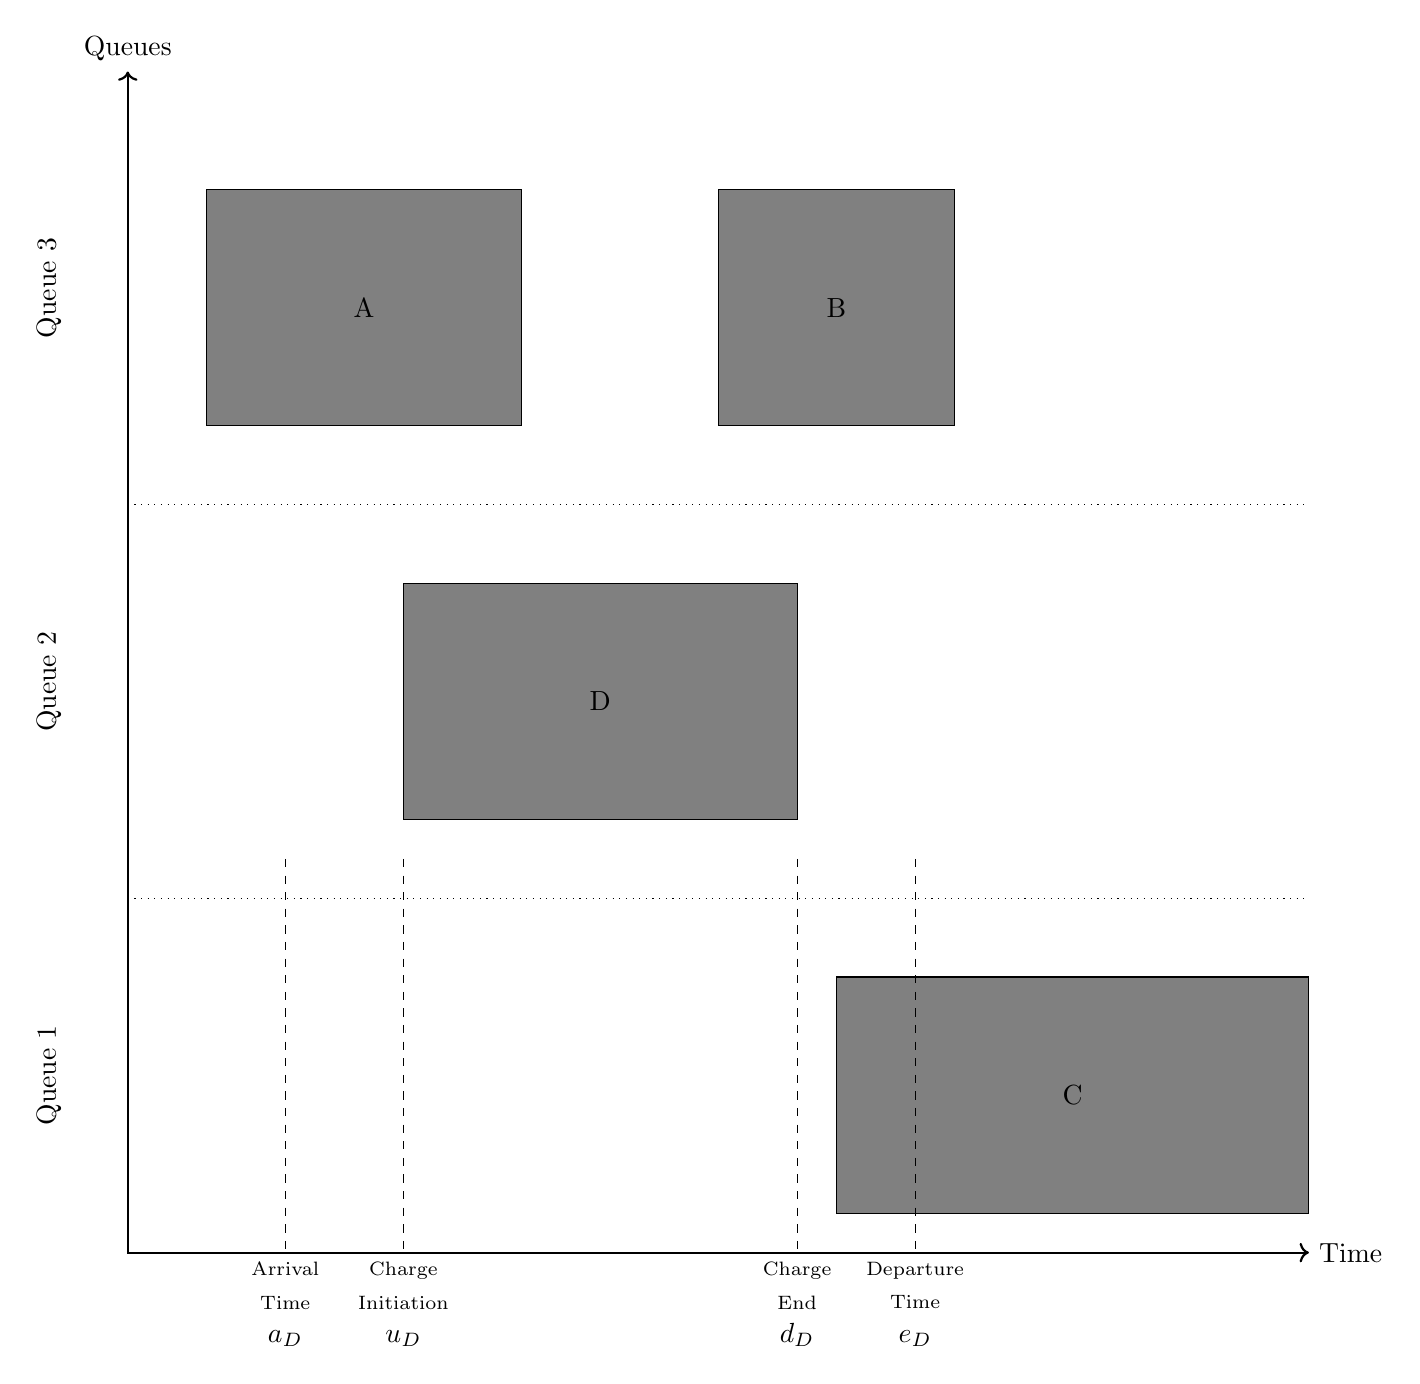
\begin{tikzpicture}
      % Variables
      \def \arrx   {2.0}
      \def \initx  {3.5}
      \def \endx   {8.5}
      \def \depx   {10.0}
      \def \yshift {5}

      % Axis
      \draw [thick,<->] (0,15) node[above]{Queues} -- (0,0) -- (15,0) node[right]{Time};

      % Rectangles
      \node[rectangle, draw, fill=gray, minimum width=4cm, minimum height = 3cm] at (3,12) {A};
      \node[rectangle, draw, fill=gray, minimum width=3cm, minimum height = 3cm] at (9,12) {B};
      \node[rectangle, draw, fill=gray, minimum width=5cm, minimum height = 3cm] at (6,7) {D};
      \node[rectangle, draw, fill=gray, minimum width=6cm, minimum height = 3cm] at (12,2) {C};

      % X-axis labels
      \node [below,align=center] at (\arrx,0) {\scriptsize Arrival     \\ \scriptsize Time \\ $a_D$};
      \node [below, align=center] at (\initx,0) {\scriptsize Charge    \\ \scriptsize Initiation  \\ $u_D$};
      \node [below, align=center] at (\endx,0) {\scriptsize Charge     \\ \scriptsize End \\ $d_D$};
      \node [below, align=center] at (\depx,0) {\scriptsize Departure  \\ \scriptsize Time \\ $e_D$};

      % Y-axis labels
      \node[rotate=90] at (-1, 2.25) {Queue 1};
      \node[rotate=90] at (-1, 7.25) {Queue 2};
      \node[rotate=90] at (-1, 12.25) {Queue 3};

      % Vertical lines
      \draw[dashed] (\arrx,\yshift)--(\arrx,0);
      \draw[dashed] (\initx,\yshift)--(\initx,0);
      \draw[dashed] (\endx,\yshift)--(\endx,0);
      \draw[dashed] (\depx,\yshift)--(\depx,0);

      % Horizontal lines
      \draw[dotted] (0, 4.5) -- (15, 4.5);
      \draw[dotted] (0, 9.5) -- (15, 9.5);

    \end{tikzpicture}
  }}
  \caption{The representation of the queue-time space. The x and y-axis represent time and space, respectively. Along the y-axis, the dashed lines represent discrete queuing locations. The shaded rectangles represent schedules BEBs to be charged. The height of each shaded rectangle represents the space taken on the queue and the width being the time to service said BEB. The vertical dashed lines are associated with vessel D and represent the arrival time, initial charge time, charge completion time, and departure time. Note that the arrival time may be before the initial charge time and the completion time may before the departure time.}
  \label{fig:spacial-and-temporal-constr}
\end{figure}

\section{Mixed Integer Linear Programming}
\label{sec:org529d812}

\begin{subequations}
\label{eq:milp-structure}
\begin{align}
&\text{max}        &J = \sum_j c_j x_j + \sum_k d_k y_k&         &               &\label{eq:fuzzy-milp-objective}\\
&\text{subject to} &\sum_j a_{ij} x_j + \sum_k g_{ik} y_k \le b_i&  &(i = 1,2,...,m)& \label{eq:fuzzy-milp-constraint}\\
&                  &x_j \ge 0&                              &(j = 1,2,...,n)& \label{eq:fuzzy-milp-continuous}\\
&                  &y_k \in \mathbb{Z^+}&                   &(k = 1,2,...,n)& \label{eq:fuzzy-milp-integer}\\
&\end{align}
\end{subequations}

The objective function in \ref{eq:fuzzy-milp-objective} comprises two parts, the continuous part, \(\sum_j c_j x_j\), and
integer part, \(\sum_k d_k y_k\). The decision variable of the first part, \(x_j\), is continuous whereas the decision variable
of the second, \(y_j\), is integer. Their respective input parameters may be integer or continuous, in the case of this
example they are modeled as continuous. The objective function's utility is to provide a numerical score to a system
(provided that a set of decision variables and input parameters are defined). While an individual score may not have any
intrinsic meaning, it provides a method of ranking different solutions of the same model. The constraint equations
(\ref{eq:fuzzy-milp-constraint} - \ref{eq:fuzzy-milp-integer}) must all be satisfied for the output of an objective
function to have any meaning. Thus, the constraint equations limit the solution space of the decision variables.
\ref{eq:fuzzy-milp-constraint} states that the summation of the products of the respective continuous and integer
decision variables and input parameters must be less than or equal to some value \(b_i\). \ref{eq:fuzzy-milp-continuous}
and \ref{eq:fuzzy-milp-integer} state that the decision variables \(x_j\) and \(y_k\), must be greater than or equal to 0,
respectively.

\section{Overview of the BAP}
\label{sec:overview-of-the-bap}
%% Rectangle packing figure
\begin{figure}
  \centering
  \includegraphics{sup-doc/milp-pap-paper-frontiers/img/spatiotemporal-packing}
  \caption{Example of rectangle packing problem. The large square represented by $O$ indicates the canstrained area that the set of shaded rectangles $\mathbb{O}$ must be placed within.}
  \label{fig:packexample}
\end{figure}

%% BAP/PAP solution plot example
\begin{figure}
  \centering
  \includegraphics{sup-doc/milp-pap-paper-frontiers/img/baprep}
  \caption{The representation of the berth-time space. The x and y-axis represent time and space, respectively. Along the y-axis, the dashed lines represent discrete berthing locations. These locations may be chosen to be continuous. The shaded rectangles represent scheduled vessels to be serviced. The height of each shaded rectangle represents the space taken on the berth and the width being the time to service said vessel. The vertical dashed lines are associated with vessel D and represent the arrival time, berthing time, serviced completion time, and departure time. Note that the arrival time may be before the berthing time and the completion time may before the departure time.}
  \label{fig:bap}
\end{figure}

The BAP is a rectangle packing problem where a set of rectangles, \(\mathbb{O}\), are attempted to be optimally placed in
a larger rectangle, \(O\), as shown in \autoref{fig:packexample}. The rectangle packing problem is an NP-hard problem that
can be used to describe many real-life problems \cite{bruin-2013-rectan-packin,murata-1995-rectan}. In some of these
problems, the dimensions of \(\mathbb{O}\) are held constant such as in the problem of packing modules on a chip, where
the widths and height of the rectangles represent the physical width and heights of the modules
\cite{murata-1995-rectan}. Other problems, such as the one presented in this work, allow either the horizontal or
vertical edge of each rectangle in \(\mathbb{O}\) to vary. As an example, suppose the vessel lengths are predefined
(vertical edges are static), but the service time is allowed to vary (horizontal edges are dynamic).
\cite{buhrkal-2011-model-discr}.

The BAP solves the problem of optimally assigning incoming vessels to berth positions to be serviced as shown in
\autoref{subfig:bapexample}. To relate to the rectangle packing problem, the width and height of \(O\) represent the time
horizon \(T\) seconds and the berth length \(L\) meters, respectively. Similarly, the widths and heights of each element in
\(\mathbb{O}\) represent the time spent to service vessel \(i\) and the space taken by docking vessel \(i\), respectively. In
the BAP, the vessel characteristics (length of the vessel, arrival time, handling time, desired departure time) are
assumed to be known for all vessels. A representation of a BAP solution is shown in \autoref{fig:bap}. The x and y-axis
represent time horizon and berthing space, respectively. The gray squares, labeled A, B, C, and D, represent berthed
vessels. The width of the boxes represents the time spent being serviced, and the height represents the amount of space
the vessel requires on the berth. The vertical line adjacent to ``Arrival Time'' represents the actual time that the
vessel arrives and is available to be berthed. ``Berthing Time'' is the time the vessel is berthed and begins being
serviced. ``Completion time'' represents the time at which the berthing space becomes available again.

\section{Overview of the PAP}
\label{sec:overview-of-the-pap}
The BAP defines the foundation of the PAP; however, there are some differences in the way the variables are interpreted. For
the \(i^{th}\) visit, starting service time is now the starting charge time, the berth location is now the charger queue
for assignment, and the service time is now the elapsed charge time. There are also a few clarifying concepts about how
the system is modeled. The PAP models the set of chargers as one continuous line; that is, the natural behavior of the
PAP model is to allow vehicles to be queued anywhere along the ``charge strip'' \([0,S]\). Similarly, the charge times are
continuous and can be placed anywhere on the time horizon, \([0,T]\), as long as the allocated times do not interfere with
other scheduled charge times.

\subsubsection{The PAP Formulation}
\label{sec:the-pap-formulation}
The BAP forms the basis of the PAP; however, there are some differences in the way the variables are interpreted. The
starting service time, \(u_i\) seconds, is viewed as the initial charge time, and the service time, total elapsed time
spent on the charger. Similarly, for the spatial term, \(v_i \in [0,L]\), the berth location is instead interpreted as the
initial position on the charger. There are also a few clarifying concepts about how the system is modeled. The PAP
models the set of chargers as one continuous line; that is, the natural behavior of the PAP model is to allow vehicles
to be queued anywhere along \([0,L]\). Similarly, the charge times are continuous and can be placed anywhere on the time
horizon, \([0,T]\), as long as the allocated times do not interfere with other scheduled charge times.

The PAP formulation's parameters can be divided into two categories: input parameters and decision variables. Each type
will now be introduced in turn. The following parameters are assumed to be known inputs for the MILP. \(L\) defines the
length of the charger in meters. As stated previously, it is modeled as a continuous bar meaninng that a vehicle can be
placed anywhere in the range \([0,L]\). It is assumed that the time horizon, \(T\) seconds, is known so that vehicles may be
placed temporarily in the range \([0,T]\). The total number of visits to the station over the time horizon is represented
by \(n_V\). The arrival time for each visit is represented by \(a_i\) seconds, and the required charge time is represented
by \(s_i\) seconds. The width of vehicle \(i\) is represented by \(l_i\) meters.

The decision variables provide the means by which the solver may optimize the problem. The initial and final charge
times for vehicle \(i\) are \(u_i\) and \(d_i\) seconds, respectively. The starting position on the charger is denoted as \(v_i
\in [0,L]\) meters. The temporal ordering of vehicles \(i\) and \(j\) is determined by \(\sigma_{ij} \in \{0, 1\}\), where \(\sigma_{ij} = 1
\implies\) \(i\) arrives before \(j\) for all \(1 \le i,j \le n_V\). Similarly, \(\psi_{ij} \in \{0, 1\}\) determines the relative
position of vehicles \(i\) and \(j\) on the charger: \(\psi_{ij} = 1 \implies v_i < v_j\) for all \(1 \le i,j \le n_V\).

To determine the values for each of these decision variables, a MILP was formulated in
\cite{qarebagh-2019-optim-sched}. The formulation is shown in its entirety for completeness.
The problem to be solved is

\begin{equation}
	\label{eq:bapobjective}
	\min\; \sum_{i=1}^N (d_i - a_i)
\end{equation}

Subject to:
\begin{subequations}
\label{eq:bapconstrs}
\begin{align}
    u_j - u_i - s_i - (\sigma_{ij} - 1)T \geq 0   \label{subeq:baptime}          \\
    v_j - v_i - l_i - (\psi_{ij} - 1)L \geq 0   \label{subeq:bapspace}           \\
    \sigma_{ij} + \sigma_{ji} + \psi_{ij} + \psi_{ji} \geq 1 \label{subeq:bapvalid_pos}     \\
    \sigma_{ij} + \sigma_{ji} \leq 1                   \label{subeq:bapsigma}        \\
    \psi_{ij} + \psi_{ji} \leq 1                   \label{subeq:bapdelta}        \\
    s_i + u_i = d_i                       \label{subeq:bapdetach}       \\
    a_i \leq u_i \leq (T - s_i)                 \label{subeq:bapvalid_starts} \\
    \sigma_{ij} \in \{0,1\},\;\psi_{ij} \in \{0,1\}\; \label{subeq:bapsdspace}      \\
    v_i \in [0, L ]                         \label{subeq:bapvspace}
\end{align}
\end{subequations}

\noindent The objective function, \autoref{eq:bapobjective}, minimizes the idle and service time by summing over the
differences between the departure time, \(d_i\), and arrival time, \(a_i\) for all visits. In other words, the objective
function is searching for the schedule that removes each vehicle from the service queue as quickly as possible.

\autoref{subeq:baptime}-\autoref{subeq:bapdelta} are used to ensure that individual rectangles do not overlap. In terms
of the PAP, this implies that there are no conflicts in the schedule spatially or temporally. \autoref{subeq:baptime}
establishes temporal ordering when active (\(\sigma_{ij}=1\)) in the manner described previously by utilizing big-M notation.
Similarly, \autoref{subeq:bapspace} establishes spatial ordering when active (\(\psi_{ij} =1\)). Constraints
\autoref{subeq:bapvalid_pos}-\autoref{subeq:bapdelta} enforce spatial and temporal ordering between each queue/vehicle
pair. Constraints \autoref{subeq:bapsigma} and \autoref{subeq:bapdelta} enforce validity of the assignments. For
example, if \autoref{subeq:bapsigma} resulted in a value of two, that would imply both vehicle \(i\) and \(j\) are scheduled
before and after each other temporally, which is impossible. In the case of \{\autoref{subeq:bapdelta}\} being equal to
two, that would mean that vehicles \(i\) and \(j\) are scheduled both before and after one another on the charging strip,
which is again impossible.\}\}

The last constraints force relationships between arrival time, initial charge time, and departure time.
\autoref{subeq:bapdetach} states that the initial charge time, \(u_i\), plus the total charge time for, \(s_i\), must equal
the departure time, \(d_i\). \autoref{subeq:bapvalid_starts} enforces the arrival time, \(a_i\), to be less than or equal to
the service start time, \(u_i\), which in turn must be less than or equal to the latest time the vehicle may begin
charging and stay within the time horizon. \autoref{subeq:bapsdspace} simply states that \(\sigma_{ij}\) and \(\psi_{ij}\) are
binary terms. \autoref{subeq:bapvspace} ensures that the assigned value of \(v_i\) is within the range, \([0,L]\).

\section{Summary}
\label{sec:org9b53a1a}
In this section the state of the art for BEB charging was discussed. The various problems of interest and solution
methods for charging BEBs were outlined. Specifically this included: BEB assignment, infrastructure optimization,
charge modeling, robust modeling, and the BAP/PAP model. The problem description for the proposed work was then provided
along with a short introduction to MILP, the BAP, and the PAP along with its formulation.
\chapter{MILP PAP}
\label{sec:milp-pap}
\section{Introduction}
\label{sec:milp-introduction}
The public transportation system is crucial in any urban area; however, the increased awareness and concern of the
environmental impacts of petroleum-based public transportation has driven an effort to reduce the pollutant footprint
\cite{de-2014-simul-elect,xylia-2018-role-charg,guida-2017-zeeus-repor-europ,li-2016-batter-elect}. Particularly,
the electrification of public bus transportation via battery power, i.e., battery-electric buses (BEBs), have received
significant attention \cite{li-2016-batter-elect}. Although the technology provides benefits beyond a reduction in
emissions, such as lower driving costs, lower maintenance costs, and reduced vehicle noise, battery-powered systems
introduce new challenges such as larger upfront costs, and potentially several hours long ``refueling'' periods
\cite{xylia-2018-role-charg,li-2016-batter-elect}. Furthermore, the problem is exacerbated by the constraints of the
transit schedule to which the fleet must adhere, the limited amount of chargers available, and the adverse effects on
the health of the battery due to fast charging \cite{lutsey-2019-updat-elect}. This paper presents a
framework for optimally assiging BEBs to charging queues assuming fixed routes while taking into consideration multiple
charger types and utilizing linear charging dynamics. This method also enforces the SOC to stay above a specified
percentage throughout the day, and ensures a minumum SOC at the end of the working day.

Many recent efforts have been made to simultaneously solve the problems of route scheduling, charging fleets, and
determining the infrastructure upon which they rely, e.g., \cite{wei-2018-optim-spatio,sebastiani-2016-evaluat-elect,hoke-2014-accoun-lithium,wang-2017-elect-vehic}. Several simplifications are made to make these problems
computationally feasible. Simplifications to the charge scheduling model include utilizing only fast chargers while
planning \cite{wei-2018-optim-spatio,sebastiani-2016-evaluat-elect,wang-2017-optim-rechar,zhou-2020-bi-objec,yang-2018-charg-sched,wang-2017-elect-vehic,qin-2016-numer-analy,liu-2020-batter-elect}. If slow chargers are used,
they are only employed at the depot and not the station \cite{he-2020-optim-charg,tang-2019-robus-sched}. Some
approaches also simplify by assuming a full charge is always achieved
\cite{wei-2018-optim-spatio,wang-2017-elect-vehic,zhou-2020-bi-objec,wang-2017-optim-rechar}. Others have assumed
that the charge received is proportional to the time spent on the charger
\cite{liu-2020-batter-elect,yang-2018-charg-sched}, which can be a valid assumption when the battery state-of-charge
(SOC) is below 80\% \cite{liu-2020-batter-elect}.

This work builds upon the Position Allocation Problem (PAP) \cite{qarebagh-2019-optim-sched}, a modification of the
well-studied Berth Allocation Problem (BAP), as a means to schedule the charging of electric vehicles
\cite{buhrkal-2011-model-discr,frojan-2015-contin-berth,imai-2001-dynam-berth}. The BAP is a continuous time model
that solves the problem of allocating space for incoming vessels to be berthed and serviced. Each arriving vessel
requires both time and space to be serviced and thus must be carefully assigned to avoid delay
\cite{imai-2001-dynam-berth}. Vessels are lined up parallel to the berth to be serviced and are horizontally queued as
shown in \autoref{subfig:bapexample}. As the vessels are serviced, they move from left to right to make space for the
queued vessels moving vertically downward into their respective berthing locations. The PAP utilizes this notion of
queuing for scheduling vehicles to be charged, as shown in \autoref{subfig:papexample}. The vehicles are queued in
several lines and move from left to right to recieve their charge and exit the system. The PAP is formulated as a
rectangle packing problem and assumes that each vehicle has a predefined charge time, the amount of vehicles that can
charge at any given moment is limited by the physical width of each vehicle and the length of the charging block. The
PAP also makes the assumption that each vehicle that is placed in the system is unique
\cite{qarebagh-2019-optim-sched}.

The main contribution of this work is the extension of the PAP's novel approach to BEB charger scheduling. This
incorporates a proportional charging model into the MILP framework, includes consideration for multiple charger types,
and consideration of each route in the schedule. The last contribution is of importance because both the BAP and PAP
consider each arrival to be unique; thus, the tracking of battery charge from one visit to the next must be considered.
Furthermore, the input parameters for the model can be predefined in such a manner as to minimize the number of fast and
slow chargers utilized as well as minimize the energy consumption. That is, the model will simultaneously minimize the
number of chargers as well as the total consumed energy. The result is a MILP formulation that coordinates charging
times and charger type for every visit while considering a dynamic charge model with scheduling constraints.

The remainder of the paper proceeds as follows: In \autoref{sec:the-position-allocation-problem}, the PAP is introduced
with a formulation of the resulting MILP. \autoref{sec:problemformulation} constructs the MILP for BEB scheduling,
including modifications to the PAP queuing constraints and the development of a dynamic charging model.
\autoref{sec:example} demonstrates an example of using the formulation to coordinate \A buses over \N total visits to
the station. The paper ends in \autoref{sec:conclusion} with concluding remarks.

\section{Position Allocation Problem}
\label{sec:the-position-allocation-problem}
This section provides a brief overview of the BAP and a detailed formulation of PAP as presented in
\cite{qarebagh-2019-optim-sched}.

\subsection{Overview of BAP}
\label{sec:overview-of-bap}
The BAP is a rectangle packing problem where a set of rectangles, \(\mathbb{O}\), are attempted to be optimally placed in
a larger rectangle, \(O\), as shown in \autoref{fig:packexample}. The rectangle packing problem is an NP-hard problem that
can be used to describe many real-life problems \cite{bruin-2013-rectan-packin,murata-1995-rectan}. In some of these
problems, the dimensions of \(\mathbb{O}\) are held constant such as in the problem of packing modules on a chip, where
the widths and height of the rectangles represent the physical width and heights of the modules
\cite{murata-1995-rectan}. Other problems, such as the one presented in this work, allow either the horizontal or
vertical edge of each rectangle in \(\mathbb{O}\) to vary. As an example, suppose the vessel lengths are predefined
(vertical edges are static), but the service time is allowed to vary (horizontal edges are dynamic).
\cite{buhrkal-2011-model-discr}.

The BAP solves the problem of optimally assigning incoming vessels to berth positions to be serviced as shown in
\autoref{subfig:bapexample}. To relate to the rectangle packing problem, the width and height of \(O\) represent the time
horizon \(T\) seconds and the berth length \(L\) meters, respectively. Similarly, the widths and heights of each element in
\(\mathbb{O}\) represent the time spent to service vessel \(i\) and the space taken by docking vessel \(i\), respectively. In
the BAP, the vessel characteristics (length of the vessel, arrival time, handling time, desired departure time) are
assumed to be known for all vessels. A representation of a BAP solution is shown in \autoref{fig:bap}. The x and y-axis
represent time horizon and berthing space, respectively. The gray squares, labeled A, B, C, and D, represent berthed
vessels. The width of the boxes represents the time spent being serviced, and the height represents the amount of space
the vessel requires on the berth. The vertical line adjacent to ``Arrival Time'' represents the actual time that the
vessel arrives and is available to be berthed. ``Berthing Time'' is the time the vessel is berthed and begins being
serviced. ``Completion time'' represents the time at which the berthing space becomes available again.

\subsection{The PAP Formulation}
\label{sec:the-pap-formulation}
The BAP forms the basis of the PAP; however, there are some differences in the way the variables are interpreted. The
starting service time, \(u_i\) seconds, is viewed as the initial charge time, and the service time, total elapsed time
spent on the charger. Similarly, for the spatial term, \(v_i \in [0,L]\), the berth location is instead interpreted as the
initial position on the charger. There are also a few clarifying concepts about how the system is modeled. The PAP
models the set of chargers as one continuous line; that is, the natural behavior of the PAP model is to allow vehicles
to be queued anywhere along \([0,L]\). Similarly, the charge times are continuous and can be placed anywhere on the time
horizon, \([0,T]\), as long as the allocated times do not interfere with other scheduled charge times.

The PAP formulation's parameters can be divided into two categories: input parameters and decision variables. Each type
will now be introduced in turn. The following parameters are assumed to be known inputs for the MILP. \(L\) defines the
length of the charger in meters. As stated previously, it is modeled as a continuous bar meaninng that a vehicle can be
placed anywhere in the range \([0,L]\). It is assumed that the time horizon, \(T\) seconds, is known so that vehicles may be
placed temporarily in the range \([0,T]\). The total number of visits to the station over the time horizon is represented
by \(n_V\). The arrival time for each visit is represented by \(a_i\) seconds, and the required charge time is represented
by \(s_i\) seconds. The width of vehicle \(i\) is represented by \(l_i\) meters.

The decision variables provide the means by which the solver may optimize the problem. The initial and final charge
times for vehicle \(i\) are \(u_i\) and \(d_i\) seconds, respectively. The starting position on the charger is denoted as \(v_i
\in [0,L]\) meters. The temporal ordering of vehicles \(i\) and \(j\) is determined by \(\sigma_{ij} \in \{0, 1\}\), where \(\sigma_{ij} = 1
\implies\) \(i\) arrives before \(j\) for all \(1 \le i,j \le n_V\). Similarly, \(\psi_{ij} \in \{0, 1\}\) determines the relative
position of vehicles \(i\) and \(j\) on the charger: \(\psi_{ij} = 1 \implies v_i < v_j\) for all \(1 \le i,j \le n_V\).

To determine the values for each of these decision variables, a MILP was formulated in
\cite{qarebagh-2019-optim-sched}. The formulation is shown in its entirety for completeness.
The problem to be solved is

\begin{equation}
	\label{eq:bapobjective}
	\min\; \sum_{i=1}^N (d_i - a_i)
\end{equation}

Subject to:
\begin{subequations}
\label{eq:bapconstrs}
\begin{align}
    u_j - u_i - s_i - (\sigma_{ij} - 1)T \geq 0   \label{subeq:baptime}          \\
    v_j - v_i - l_i - (\psi_{ij} - 1)L \geq 0   \label{subeq:bapspace}           \\
    \sigma_{ij} + \sigma_{ji} + \psi_{ij} + \psi_{ji} \geq 1 \label{subeq:bapvalid_pos}     \\
    \sigma_{ij} + \sigma_{ji} \leq 1                   \label{subeq:bapsigma}        \\
    \psi_{ij} + \psi_{ji} \leq 1                   \label{subeq:bapdelta}        \\
    s_i + u_i = d_i                       \label{subeq:bapdetach}       \\
    a_i \leq u_i \leq (T - s_i)                 \label{subeq:bapvalid_starts} \\
    \sigma_{ij} \in \{0,1\},\;\psi_{ij} \in \{0,1\}\; \label{subeq:bapsdspace}      \\
    v_i \in [0, L ]                         \label{subeq:bapvspace}
\end{align}
\end{subequations}

\noindent The objective function, \autoref{eq:bapobjective}, minimizes the idle and service time by summing over the
differences between the departure time, \(d_i\), and arrival time, \(a_i\) for all visits. In other words, the objective
function is searching for the schedule that removes each vehicle from the service queue as quickly as possible.

\autoref{subeq:baptime}-\autoref{subeq:bapdelta} are used to ensure that individual rectangles do not overlap. In terms
of the PAP, this implies that there are no conflicts in the schedule spatially or temporally. \autoref{subeq:baptime}
establishes temporal ordering when active (\(\sigma_{ij}=1\)) in the manner described previously by utilizing big-M notation.
Similarly, \autoref{subeq:bapspace} establishes spatial ordering when active (\(\psi_{ij} =1\)). Constraints
\autoref{subeq:bapvalid_pos}-\autoref{subeq:bapdelta} enforce spatial and temporal ordering between each queue/vehicle
pair. Constraints \autoref{subeq:bapsigma} and \autoref{subeq:bapdelta} enforce validity of the assignments. For
example, if \autoref{subeq:bapsigma} resulted in a value of two, that would imply both vehicle \(i\) and \(j\) are scheduled
before and after each other temporally, which is impossible. In the case of \{\autoref{subeq:bapdelta}\} being equal to
two, that would mean that vehicles \(i\) and \(j\) are scheduled both before and after one another on the charging strip,
which is again impossible.\}\}

The last constraints force relationships between arrival time, initial charge time, and departure time.
\autoref{subeq:bapdetach} states that the initial charge time, \(u_i\), plus the total charge time for, \(s_i\), must equal
the departure time, \(d_i\). \autoref{subeq:bapvalid_starts} enforces the arrival time, \(a_i\), to be less than or equal to
the service start time, \(u_i\), which in turn must be less than or equal to the latest time the vehicle may begin
charging and stay within the time horizon. \autoref{subeq:bapsdspace} simply states that \(\sigma_{ij}\) and \(\psi_{ij}\) are
binary terms. \autoref{subeq:bapvspace} ensures that the assigned value of \(v_i\) is within the range, \([0,L]\).

\section{A Rectangle Packing Formulation for BEB Charging}
\label{sec:problemformulation}
Applying the PAP to BEB charging requires four fundamental changes. The first is that the time that a BEB spends
charging must be allowed to vary. That is, \(u_i\), \(d_i\), and \(s_i\) become variables of optimization. This is done
primarily because chargers of various speeds are to be introduced. Allowing BEBs to have multiple visits that a charger
decided upon during the optimization requires that the start and stop times must be changeable to respect the SOC
constraints. Second, in the PAP each visit is assumed to be a different vehicle. For the BEB charging problem, each bus
may make multiple visits to the station throughout the day. Thus, the resulting SOC for a bus at a given visit is
dependent upon each of the prior visits. The third fundamental change is related to the first two. The SOC of each bus
must be tracked to ensure that charging across multiple visits is sufficient to allow each bus to execute its route
throughout the day. Finally, as previously stated, the PAP models the charger as one continuous bar. For the BEB, it
will be assumed that a discrete number of chargers exist. Moreover, it is assumed that these chargers may have different
charge rates.

A few assumptions are made in the derivation of the algorithm. As this work is not focused on estimating the discharge
of a BEB during its route, the discharge for each route will be pre-calculated by assuming a fixed discharge rate kW
multiplied by the route duration in hours. Secondly, it is assumed that the initial SOC of each BEB at the beginning of
the day, $\alpha_b\kappa_b$, is larger than the minimum required SOC at the end of the day, $\beta_b\kappa_b$.
Therefore, it must be assumed that the difference in the SOC can reach $\alpha_b\kappa_b$ by the beginning of the next
working day.

The discussion of the four changes is separated into two sections. \autoref{sec:queuing} discusses the changes in the
spatial-temporal constraint formulation to form a queuing constraint. \autoref{sec:batt_dynamics} then discusses the
addition of bus charge management. This section ends with a brief discussion of a modified objective function and the
statement of the full problem in \autoref{sec:BEB_MILP}. The notation is explained throughout and summarized in
\autoref{tab:variables}.

\subsection{Queuing Constraints}
\label{sec:queuing}
\noindent The queuing constraints ensure that the buses entering the charging queues are assigned
feasibly. There are three sets to differentiate between different entities. \(\mathbb{B} = \{1, ..., n_B\}\) is the set of
bus indices with index \(b\) used to denote an individual bus, \(\mathbb{Q} = \{1, ..., n_Q\}\) is the set of queues with index \(q\)
used to denote an individual queue, and \(\mathbb{V} = \{1, ..., n_V\}\) is a set of visits to the station with \(i\) and
\(j\) used to refer to individual visits. The mapping \(\Gamma: \mathbb{V} \rightarrow \mathbb{B}\) is used to map a visit
index, \(i\), to a bus index, \(b\). The notation \(\Gamma_i\) is used as a shorthand to refer to the bus index \(b\) for visit
\(i\).

The actual physical dimensions of the BEB are ignored and it is assumed that each BEB will be assigned to charge at a
particular charger. Because of this assumption, the PAP spatial variable, \(l_i\), may be removed and \(v_i\) is made to be
an integer corresponding to which queue visit \(i\) will be using, \(v_i \in \mathbb{Q}\). That is, the queue position is now
discretized over \(n_Q\) chargers where a BEB occupies single charge queue. Thus, when \(\psi_{ij} = 1\), vehicle \(j\) is placed
in a charging queue with a larger index than vehicle \(i\), \(v_j > v_i\). The charger length \(L\) is likewise replaced with
\(n_Q\). Note that \(n_Q = n_B + n_C\), where \(n_B\) is the number of buses and \(n_C\) is the number of chargers. The
rationale for adding additional idle queues is to allow BEBs to be ``set aside'' if no additional charge is required.
Adding one idle queue for each BEB ensures that the constraints will be satisfied if multiple buses sharing overlapping
times at the station are placed in idle queues. This method will be applied when defining the parameters in
\{\autoref{sec:example}\}. The modified queuing constraints can be written as shown in \autoref{eq:packconstrs}.

\begin{subequations}
\label{eq:packconstrs}
\begin{align}
    v_i - v_j - (\psi_{ij} - 1)n_Q \geq 1 \label{subeq:space} \\ d_i \leq \tau_i \label{subeq:valid_depart} \\ s_i \geq
    0 \label{subeq:pos_charge} \\ v_i \in \mathbb{Q} \label{subeq:vspace}
\end{align}
\end{subequations}

The constraint in \autoref{subeq:space} is nearly identical to \autoref{subeq:bapspace}, but rather than viewing the
charger as a continuous strip of length \(S\), it is discretized into \(n_Q\) queues each with a width of unit length one. A
BEB is also assigned a unit length of one which is reflected in \autoref{subeq:space} by \(\cdot \geq 1\).
\autoref{subeq:valid_depart} ensures that the time the BEB is detached from the charger, \(d_i\), is before its departure
time, \(\tau_i\) seconds. Note the introduction of the new variable \(\tau_i\) exists to allow the final charge time to be
independent a similar manner that the inital charge time need not coincide with the arrival time, \(a_i \le u_i \le d_i \le
\tau_i\). \autoref{subeq:vspace} defines the of integers that \(v_i\) that represent the \(n_Q\) chargers.

\subsection{Battery Charge Dynamic Constraints}
\label{sec:batt_dynamics}
Battery dynamic constraints are now to be introduced. Two constraints are enforced on the SOC for each BEB: the SOC must
always remain above a specified percentage to guarantee sufficient charge to execute their respective routes and each
bus must end the day with an SOC above a specified threshold, preparatory for the next day.

The SOC upon arrival for visit \(i\) is denoted as \(\eta_i\) kWh. Because the SOC for a visit \(i\) is dependent on its previous
visits, the mapping \(\Upsilon: \mathbb{V} \rightarrow \mathbb{V} \bigcup \{\varnothing\}\) is used to determine the next visit that corresponds
to the same bus, with \(\Upsilon_i\) being shorthand notation. Thus, \(\Gamma_j\) and \(\Gamma_{\Upsilon_i}\), for \(\Upsilon_i = j\), would both map to the
same bus index as long as \(\Upsilon_i\) is not the null element, \(\varnothing\). The null element is reserved for BEBs that have
no future visits.

To drive time spent on the charger, $s_i$, as well as define initial, final, and intermediate bus charges for each visit
$i$, the sets for initial and final visits must be defined. Let the mapping of the first visit by each bus be denoted as
$\Gamma^0 : \mathbb{B} \rightarrow \mathbb{V}$. The resulting value of the mapping $\Gamma^0$ represents the index for
the first visit of bus $b$. Similarly, let $\Gamma^f : \mathbb{B} \rightarrow \mathbb{V}$ maps the indices for the final
visits for each bus $b \in \mathbb{B}$. Let the storthand for each mapping be denoted as $\Gamma^0_b$ and $\Gamma^f_b$,
respectively. The initial and final bus charge percentages, $\alpha$ and $\beta$, can then be represented by the
constraint equations $\eta_{\Gamma^0_b} = \alpha_b \kappa_{b}$ and $\eta_{\Gamma^f_b} = \beta_b \kappa_{b}$,
respectively. The intermediate charges must be determined during runtime.

It is assumed that the charge received is proportional to the time spent charging. The rate for charger \(q\) is denoted
as \(r_q\) kW. Note that a value of \(r_q = 0\) corresponds to a queue where no charging occurs. A bus in such a queue is
simply waiting at the station for the departure time. The queue indices are ordered such that the first \(n_B\) queues
have \(r_q = 0\) to allow an arbitrary number of buses to sit idle at any given moment in time. The next \(n_C\) queues are
reserved for the slow and fast chargers. The amount of discharge between visits \(i\) and \(\Upsilon_i\), the next visit of the
same bus, is denoted as \(\Delta_i\) kWh. If visit \(i\) occurred at charger \(q\), the SOC of the BEB's next arrival, \(\Upsilon_i\), would
be \(\eta_{\Upsilon_i} = \eta_i + s_i r_q - \Delta_i\).

The binary decision variable \(w_{iq} \in \{0,1\}\) is introduced to indicate the active charger for visit \(i\) in vector
form. The form of the SOC for the next visit, \(\Upsilon_i\), can be written using the following constraints.

\begin{subequations}
    \label{subeq:pre_next_charge}
\begin{align}
    \eta_{\Upsilon_i} = \eta_i + \sum_{q=1}^{n_Q} s_i w_{iq} r_q - \Delta_i \\
    \sum_{q=1}^{n_Q} w_{iq} = 1                           \\
    w_{iq} \in \{0,1\}.
\end{align}
\end{subequations}

The choice of queue for visit \(i\), becomes a slack variable and is defined in terms of \(w_{iq}\) as

\begin{equation}
    v_i = \sum_{q=1}^{n_Q} qw_{iq}.
\end{equation}

Maximum and minimum values for the charges are included to ensure that the battery is not overcharged and to guarantee
sufficient charge for subsequent visits. The upper and lower battery charge bounds for bus \(b\) are \(\kappa_b\) and \(\nu_b \kappa_b\),
respectively , where \(\kappa_b\) is the battery capacity and \(\nu_b\) is a percent value. The upper and lower bounds for the
current SOC are written as follows.

\begin{subequations}
    \label{subeq:pre_min_max}
\begin{align}
    \eta_i + \sum_{q=1}^{n_Q} s_i w_{iq} r_q \leq \kappa_{\Gamma_i} \label{eq:maxcharge}\\
    \eta_i \geq \nu_{\Gamma_i} \kappa_{\Gamma_i} \label{eq:mincharge}
\end{align}
\end{subequations}

\autoref{eq:maxcharge} ensures that the BEB SOC does not exceed the battery capacity, and \autoref{eq:mincharge}
enforces that the inital SOC for each visit is above the threshold of \(\nu_{\Gamma_i}\kappa_{\Gamma_i}\). Note that the term \(s_i w_{iq}\)
is a bilinear term. A standard way of linearizing a bilinear term that contains an integer variable is by introducing a
slack variable with an either/or constraint \cite{chen-2010-applied,rodriguez-2013-compar-asses}. Allowing the slack
variable \(g_{iq}\) seconds to be equal to \(s_i w_{iq}\), \(g_{iq}\) can be defined as

\begin{equation}
    \label{eq:giq_cases}
    g_{iq} =
    \begin{cases}
        s_i & w_{iq} = 1 \\
        0 & w_{iq} = 0
    \end{cases}.
\end{equation}

\autoref{eq:giq_cases} can be expressed as a mixed integer constraint using big-M notation with the following four
constraints.

\begin{subequations}
    \label{eq:slack_gain}
\begin{align}
    s_i - (1 - w_{iq})M \leq g_{iq}  \label{subeq:repgpgret} \\
    s_i \geq g_{iq}                 \label{subeq:repgples} \\
    Mw_{iq} \geq g_{iq}              \label{subeq:repgwgret} \\
    0 \leq g_{iq}                   \label{subeq:repgwles}
\end{align}
\end{subequations}

\noindent where \(M\) is a large unitless value. If \(w_{iq} = 1\) then \autoref{subeq:repgpgret} and
\autoref{subeq:repgples} become \(s_i \leq g_{iq}\) and \(s_i \geq g_{iq}\), forcing \(s_i = g_{iq}\) with \autoref{subeq:repgwgret}
being inactive. If \(w_{iq} = 0\), \autoref{subeq:repgpgret} is inactive and \autoref{subeq:repgwgret} and
\autoref{subeq:repgwles} force \(g_{iq} = 0\).

\subsection{The BEB Charging Problem}
\label{sec:BEB_MILP}
The goal of the MILP is to utilize chargers as little as possible to reduce energy costs with fast charging being
penalized more to avoid the adverse effects of fast charging on battery health as well as the
larger usage cost. Thus, an assignment cost \(m_q\) and usage cost \(\epsilon_q\) are associated with each charger, \(q\).
These unitless weights can be adjusted based on charger type or time of day that the visit
occurs. The assignment term takes the form \(w_{iq}m_q\), and the usage term takes the form \(g_{iq} \epsilon_q\). The
resulting BEB charging problem is defined in \autoref{eq:objective}.

\begin{equation}
\label{eq:objective}
	\min \sum_{i=1}^N \sum_{q=1}^{n_Q} \Big( w_{iq} m_q + g_{iq} \epsilon_q \Big) \\
\end{equation}

Subject to the constraints

\begin{multicols}{2}
\begin{subequations}
                                                     \label{eq:dynconstrs}
\begin{equation}
    u_j - u_i - s_i - (\sigma_{ij} - 1)T \geq 0              \label{subeq:m_time}         \\
\end{equation}
\begin{equation}
    v_j - v_i - (\psi_{ij} - 1)n_Q \geq 1                  \label{subeq:m_space}        \\
\end{equation}
\begin{equation}
    \sigma_{ij} + \sigma_{ji} + \psi_{ij} + \psi_{ji} \geq 1            \label{subeq:m_valid_pos}    \\
\end{equation}
\begin{equation}
    \sigma_{ij} + \sigma_{ji} \leq 1                              \label{subeq:m_sigma}        \\
\end{equation}
\begin{equation}
    \psi_{ij} + \psi_{ji} \leq 1                              \label{subeq:m_delta}        \\
\end{equation}
\begin{equation}
    s_i + u_i = d_i                                  \label{subeq:m_detach}       \\
\end{equation}
\begin{equation}
    \eta_{\Gamma^0_b} = \alpha_{\Gamma_i} \kappa_{\Gamma_i}                         \label{subeq:init_charge}    \\
\end{equation}
\begin{equation}
    a_i \leq u_i \leq (T - s_i)                            \label{subeq:m_valid_starts} \\
\end{equation}
\begin{equation}
    d_i \leq \tau_i                                        \label{subeq:m_valid_depart} \\
\end{equation}
\begin{equation}
    \eta_i + \sum_{q=1}^{n_Q} g_{iq} r_q - \Delta_i = \eta_{\gamma_i}   \label{subeq:next_charge}    \\
\end{equation}
\begin{equation}
    \eta_i + \sum_{q=1}^{n_Q} g_{iq} r_q - \Delta_i \geq \nu_{\Gamma_i} \kappa_{\Gamma_i} \label{subeq:min_charge}     \\
\end{equation}
\begin{equation}
    \eta_i + \sum_{q=1}^{n_Q} g_{iq} r_q \leq \kappa_{\Gamma_i}         \label{subeq:max_charge}     \\
\end{equation}
\begin{equation}
    \eta_{\Gamma^f_b} \geq \beta_{\Gamma_i} \kappa_{\Gamma_i}                   \label{subeq:final_charge}   \\
\end{equation}
\begin{equation}
    s_i - (1 - w_{iq})M \leq g_{iq}                     \label{subeq:gpgret}         \\
\end{equation}
\begin{equation}
    s_i \geq g_{iq}                                     \label{subeq:gples}          \\
\end{equation}
\begin{equation}
    Mw_{iq} \geq g_{iq}                                 \label{subeq:gwgret}         \\
\end{equation}
\begin{equation}
    0 \leq g_{iq}                                       \label{subeq:gwles}          \\
\end{equation}
\begin{equation}
    v_i = \sum_{q=1}^{n_Q} qw_{iq}                      \label{subeq:wmax}           \\
\end{equation}
\begin{equation}
    \sum_{q=1}^{n_Q} w_{iq} = 1                         \label{subeq:wone}           \\
\end{equation}
\begin{equation}
   w_{iq}, \sigma_{ij}, \psi_{ij} \in \{0,1\}\;            \label{subeq:binaryspace}        \\
\end{equation}
\begin{equation}
    v_i, q_i \in  \mathbb{Q}                                         \label{subeq:Qspace}        \\
\end{equation}
\begin{equation}
    i \in \mathbb{V}                                   \label{subeq:Ispace}         \\
\end{equation}
\end{subequations}
\end{multicols}

\autoref{subeq:m_time}-\autoref{subeq:m_valid_depart} are reiterations of the queuing constraints in
\autoref{eq:packconstrs}. \autoref{subeq:init_charge}-\autoref{subeq:final_charge} provide the battery charge
constraints. \autoref{subeq:gpgret}-\autoref{subeq:gwles} define the charge gain of every visit/queue pairing. The last
constraints \autoref{subeq:binaryspace}-\autoref{subeq:Ispace} define the sets of valid values for each variable.

\section{Example}
\label{sec:milp-example}
\begin{subfigures}
    %%~~~~~~~~~~~~~~~~~~~~~~~~~~~~~~~~~~~~~~~~~~~~~~~~~~~~~~~~~~~~~~~~~~~~~~~~~~~~
    % BAP
    \begin{figure}[htpb]
    \centering
        \includestandalone{sup-doc/milp-pap-paper-frontiers/img/bap}
        \caption{Example of berth allocation. Vessels are docked in berth locations (horizontal) and are queued over
          time (vertical). The vertical arrow represents the movement direction of queued vessels and the horizontal
          arrow represents the direction of departure.}
        \label{subfig:bapexample}
    \end{figure}
    \hfill

    %%~~~~~~~~~~~~~~~~~~~~~~~~~~~~~~~~~~~~~~~~~~~~~~~~~~~~~~~~~~~~~~~~~~~~~~~~~~~~
    % PAP
    \begin{figure}[htpb]
    \centering
        \includestandalone{sup-doc/milp-pap-paper-frontiers/img/pap}
        \caption{Example of position allocation. Vehicles are placed in queues to be charged and move in the direction
          indicated by the arrow.}
        \label{subfig:papexample}
    \end{figure}
\end{subfigures}


\begin{table}[!htpb]
  \caption{Notation used throughout the paper. Units are provided when available.}
  \label{tab:variables}
  \centering
  \begin{tabularx}{\textwidth}{l l l}
    \toprule \textbf{Variable} & \textbf{Units} & \textbf{Description}                                                                      \\
    \toprule \multicolumn{3}{l}{Input values}                                                                                               \\
    \hline $n_B$ & & Number of buses                                                                                                        \\
    $M$           &       & An arbitrarily large number                                                                                     \\
    $n_V$         &       & Number of total visits                                                                                          \\
    $n_Q$         &       & Number of queues                                                                                                \\
    $n_C$         &       & Number of chargers                                                                                              \\
    $\mathbb{V}$  &       & Set of visit indices, $\mathbb{V} = \{1, ..., n_V\}$                                                            \\
    $\mathbb{B}$  &       & Set of bus indices, $\mathbb{B} = \{1, ..., n_B\}$                                                              \\
    $\mathbb{Q}$           &       & Set of queue indices, $\mathbb{Q} = \{1, ..., n_Q\}$                                                                     \\
    $i,j$         &       & Indices used to refer to visits                                                                                 \\
    $b$           &       & Index used to refer to a bus                                                                                    \\
    $q$           &       & Index used to refer to a queue                                                                                  \\
    \hline \multicolumn{3}{l}{Problem definition parameters}                                                                                \\
    \hline $\Gamma$    &       & $\Gamma: \mathbb{V} \rightarrow \mathbb{B}$ with $\Gamma_i$ used as a shorthand to denote the bus $b$ for visit $i$                 \\
    $\alpha_b$         & $\%$  & Initial charge percentage time for bus $b$                                                                      \\
    $\beta_b$         & $\%$  & Final charge percentage for bus $b$ at the end of the time horizon                                              \\
    $\epsilon_q$         &       & Cost of using charger $q$ per unit time                                                                         \\
    $\Upsilon$           &       & $\Upsilon: \mathbb{V} \rightarrow \mathbb{V}$ mapping a visit to the next visit by the same bus with $\Upsilon_i$ being the shorthand.  \\
    $\kappa_b$         & kWh   & Battery capacity for bus $b$                                                                                    \\
    $\Delta_i$         & kWh   & Discharge of visit over route $i$                                                                               \\
    $\nu_b$         & $\%$  & Minimum charge allowed for bus $b$                                                                              \\
    $\tau_i$         & s     & Time visit $i$ must depart the station                                                                          \\
    $\zeta_b$         & kW    & Discharge rate for bus $b$                                                                                      \\
    $a_i$         & s     & Arrival time of visit $i$                                                                                       \\
    $i_0$         &       & Indices associated with the initial arrival
    for every bus in $\mathbb{B}$                                                                                                           \\
    $i_f$         &       & Indices associated with the final arrival for every bus in $\mathbb{B}$                                         \\
    $m_q$         &       & Cost of a visit being assigned to charger $q$                                                                   \\
    $r_q$         & kW    & Charge rate of charger $q$ per unit time                                                                        \\
    \hline \multicolumn{3}{l}{Decision Variables}                                                                                           \\
    \hline $\psi_{ij}$          &                         & Binary variable determining spatial ordering of vehicles $i$ and $j$               \\
    $\eta_i$     & kWh  & Initial charge for visit $i$                                                                                         \\
    $\sigma_{ij}$  &      & Binary variable determining temporal ordering of vehicles $i$ and $j$                                                \\
    $d_i$     & s    & Ending charge time for visit $i$                                                                                     \\
    $g_{iq}$  & s    & Linearization term, represents the multiplication of $s_i w_{iq}$                                                     \\
    $s_i$     & s    & Amount of time spent on charger for visit $i$                                                                        \\
    $u_i$     & s    & Starting charge time of visit $i$                                                                                    \\
    $v_i$     &      & Assigned queue for visit $i$                                                                                         \\
    $w_{iq}$  &      & Binary assignment variable for visit $i$ to queue $q$                                                                \\
    \bottomrule
  \end{tabularx}
\end{table}

\begin{figure}[htpb]
\centering
    \includegraphics{sup-doc/milp-pap-paper-frontiers/img/spatiotemporal-packing}
    \caption{Example of the rectangle packing problem. The large square represented by $O$ indicates the constrained
      area that the set of shaded rectangles $\mathbb{O}$ must be placed within.}
    \label{fig:packexample}
\end{figure}

\begin{figure}[ht]
\centering
    \includegraphics{sup-doc/milp-pap-paper-frontiers/img/baprep}
    \caption{The representation of the berth-time space. The x and y-axis represent time and space, respectively. Along
      the y-axis, the dashed lines represent discrete berthing locations. These locations may be chosen to be
      continuous. The shaded rectangles represent scheduled vessels to be serviced. The height of each shaded rectangle
      represents the space taken on the berth and the width being the time to service said vessel. The vertical dashed
      lines are associated with vessel D and represent the arrival time, berthing time, service completion time, and
      departure time. Note that the arrival time may be before the berthing time and the completion time may be before
      the departure time.}
    \label{fig:bap}
\end{figure}

\begin{figure}[htpb]
\centering
    \includegraphics{sup-doc/milp-pap-paper-frontiers/img/overlap}
    \caption{Examples of different methods of overlapping. Space overlap: $v_{k_1} < v_{i} + l_i \therefore \psi_{k_{1}i} = 0$.
             Time overlap $u_{k_1} < u_{j} + s_j \therefore \sigma_{k_{2}j} = 0$. Both space and time overlap $\sigma_{k_{3}i} = 0$ and
             $\psi_{k_{3}j} = 0$.}
    \label{fig:multipleassign}
\end{figure}

\begin{subfigures}
    %%~~~~~~~~~~~~~~~~~~~~~~~~~~~~~~~~~~~~~~~~~~~~~~~~~~~~~~~~~~~~~~~~~~~~~~~~~~~~
    % Qin
    \begin{figure}[htpb]
    \centering
    \includegraphics{sup-doc/milp-pap-paper-frontiers/img/schedule-qin}
        \caption{Charging schedule generated by Qin Modified algorithm.}
        \label{subfig:qin-schedule}
    \end{figure}

    \hfill

    %%~~~~~~~~~~~~~~~~~~~~~~~~~~~~~~~~~~~~~~~~~~~~~~~~~~~~~~~~~~~~~~~~~~~~~~~~~~~~
    % MILP
    \begin{figure}[htpb]
    \centering
        \includegraphics{sup-doc/milp-pap-paper-frontiers/img/schedule-milp}
        \caption{Charging schedule generated by MILP PAP algorithm.}
        \label{subfig:milp-schedule}
    \end{figure}
\end{subfigures}

\begin{subfigures}
    %%~~~~~~~~~~~~~~~~~~~~~~~~~~~~~~~~~~~~~~~~~~~~~~~~~~~~~~~~~~~~~~~~~~~~~~~~~~~~
    % Fast
    \begin{figure}[htpb]
    \centering
        \includegraphics{sup-doc/milp-pap-paper-frontiers/img/charger-count-fast}
        \caption{Number of fast chargers for Qin and MILP PAP.}
        \label{subfig:fast-charger-usage}
    \end{figure}

    \hfill

    %%~~~~~~~~~~~~~~~~~~~~~~~~~~~~~~~~~~~~~~~~~~~~~~~~~~~~~~~~~~~~~~~~~~~~~~~~~~~~
    % Slow
    \begin{figure}[!ht]
    \centering
        \includegraphics{sup-doc/milp-pap-paper-frontiers/img/charger-count-slow}
        \caption{Number of slow chargers for Qin and MILP PAP.}
        \label{subfig:slow-charger-usage}
    \end{figure}
\end{subfigures}

\begin{subfigures}
    %%~~~~~~~~~~~~~~~~~~~~~~~~~~~~~~~~~~~~~~~~~~~~~~~~~~~~~~~~~~~~~~~~~~~~~~~~~~~~
    % Qin
    \begin{figure}[htpb]
    \centering
        \includegraphics{sup-doc/milp-pap-paper-frontiers/img/charge-qin}
        \caption{Bus charges for the Qin Modified charging schedule. The charging scheme of the Qin charger is more predictable during the working day.}
        \label{subfig:qin-charge}
    \end{figure}

    \hfill

    %%~~~~~~~~~~~~~~~~~~~~~~~~~~~~~~~~~~~~~~~~~~~~~~~~~~~~~~~~~~~~~~~~~~~~~~~~~~~~
    % MILP
    \begin{figure}[htpb]
    \centering
        \includegraphics{sup-doc/milp-pap-paper-frontiers/img/charge-milp}
        \caption{The bus charges for the MILP PAP charging schedule. The MILP model allows for guarantees of minimum/maximum changes during the working day as well as charges at the end of the day.}
        \label{subfig:milp-charge}
    \end{figure}
\end{subfigures}

\begin{figure}[htpb]
\centering
    \includegraphics{sup-doc/milp-pap-paper-frontiers/img/power}
    \caption{Amount of power consumed by Qin-Modified and MILP schedule over the time horizon.}
    \label{fig:power-usage}
\end{figure}

\begin{figure}[htpb]
\centering
    \includegraphics{sup-doc/milp-pap-paper-frontiers/img/energy}
    \caption{Total accumulated energy consumed by the Qin-Modified and MILP schedule throughout the time horizon.}
    \label{fig:energy-usage}
\end{figure}

\chapter{SA PAP}
\label{sec:sa-pap}
\section{Introduction}
\label{sec:sa-introduction}
Public transportation systems are a critical component urban areas. An increased awareness and concern of environmental
impacts of petroleum based public transportation has driven an effort to reduce the pollutant footprint
\cite{de-2014-simul-elect,xylia-2018-role-charg,guida-2017-zeeus-repor-europ,li-2016-batter-elect}. Particularly,
the electrification of public bus transportation via battery power, i.e., battery electric buses (BEBs), has received
significant attention \cite{li-2016-batter-elect}. Although the technology provides benefits beyond reduction in
emissions, such as lower driving costs, lower maintenance costs, and reduced vehicle noise, battery powered systems
introduce new challenges such as larger upfront costs, and potentially several hours long ``refueling'' periods
\cite{xylia-2018-role-charg,li-2016-batter-elect}. Furthermore, the problem is exacerbated by the constraints of the
transit schedule to which the fleet must adhere, the limited amount of chargers available, and the adverse affects in
the health of the battery due to fast charging \cite{lutsey-2019-updat-elect}. This work presents a scheduling
framework for a BEB fleet that allows for multiple charger types and partial charging. It considers linear battery
dynamics, fixed bus schedules, enforces a state-of-charge (SOC) threshold, and takes into consideration the total energy
consumed by the schedule as well as peak power use.

Literature shows an interest in solving the problem of assigning BEBs to charging queues or optimizing their
infrastructure \cite{wei-2018-optim-spatio,sebastiani-2016-evaluat-elect,hoke-2014-accoun-lithium,wang-2017-elect-vehic}. Two of the main problems that have been of recent interest are
solving the problems of route scheduling, charging fleets, and determining the infrastructure upon which they rely.
Additionally, the prospect of solving both problems simultaneously has received much attention
\cite{wei-2018-optim-spatio,sebastiani-2016-evaluat-elect,hoke-2014-accoun-lithium,wang-2017-elect-vehic}. These
problems vary by including assignment of buses to routes \cite{rinaldi-2020-mixed-fleet,zhou-2020-collab-optim,tang-2019-robus-sched,li-2014-trans-bus}, determining whether a set of existing combustion based buses should be
replaced with BEBs \cite{zhou-2020-bi-objec,duan-2021-refor-mixed,rinaldi-2020-mixed-fleet,zhou-2020-collab-optim}, and accounting for uncertainties \cite{bie-2021-optim-elect,duan-2021-refor-mixed,tang-2019-robus-sched,ursavas-2016-optim-polic}. These problems add additional complexities that warrant
simplifications due to computational complexities. One other source, as far as the reseach for this work has shown,
describes a method of producing a BEB charge schedule wih a high fidelity while accounting for multiple charger times as
well as being able to minimize over the total charger count \cite{whitaker-2023-a-network}. This work aims to focus on
day-to-day requirements which require a higher fidelity charging and scheduling models to more accurately estimate the
monetary cost of charging. Specifically, the framework to be presented creates a charging schedule for a fixed set of
bus routes while minimizing the total number of chargers required and minimizing the monetary cost of charging the BEBs
by minimizing the demand and consumption costs.

Some works assume that the charge received is proportional to the time spent on the charger
\cite{liu-2020-batter-elect,yang-2018-charg-sched}. While the linear battery dynamics is a valid assumption when the
battery SOC is below 80\% \cite{liu-2020-batter-elect}, non-linear battery dynamics can be implemented to more
accurately model the charge curve. A common way to model the non-linear battery dynamics is utilizing Constant Voltage
(CV), Constant Current (CC), and Constant Current Constant Voltage (CCCV) \cite{abdollahi-2016-optim-batter,chen-2008-desig-grey}. It has also been suggested that the dynamics can be modeled as a piecewise function containing a
linear and non-linear component from which the CV and CC models construct the linear and non-linear parts, respectively
\cite{zhang-2021-optim-elect,abdollahi-2016-optim-batter}. Others have modeled the battery dynamics as a discrete
first order dynamics model \cite{whitaker-2023-a-network}. The first-order differential system, when provided a step
input, approximates the non-linear relationship between time and SOC \cite{whitaker-2023-a-network}. While the
framework presented in this work may implement the non-linear battery dynamics model, linear battery dynamics are chosen
to allow comparisons between other solution methods.

Works concerning charge planning often use a version of the vehicle scheduling problem \cite{tang-2019-robus-sched,li-2014-trans-bus,he-2020-optim-charg}. Variants of this problem address infrastructure as well as determining
existing buses that should be replaced by a BEB \cite{zhou-2020-bi-objec,duan-2021-refor-mixed,rinaldi-2020-mixed-fleet,zhou-2020-collab-optim}. Other works introduce a directed graph approach to model the flow
of BEBs \cite{whitaker-2023-a-network,liu-2020-batter-elect}, where this concept was expanded to simultaneously
accounting for multiple charger types, partial charging, non-linear battery charge profiles
\cite{whitaker-2023-a-network}. The directed graph approach provides a simple method of modeling the scheduling by
discretizing the time horizon into a sequence of nodes for each charger. The nodes represent discrete steps in time in
which BEBs may be assigned to be charged. BEBs may be assigned to sequential time steps of a singular charger. Once it
has completed its charge, the BEB is then transitioned out of the charge queue creating an opening for another BEB to
receive charge. This work bases its implementation on what is known as the Position allocation problem
\cite{qarebagh-2019-optim-sched}.

The PAP is derived from the Berth Allocation Problem (BAP) which solves the problem of scheduling a set of vessels to be
berthed and serviced. The model inputs a set of vessels arrival and service times and outputs a schedule that defines
the selected berth and the time over which it is serviced. The PAP utilizes this model and redefines its inputs to EV
arrival times and outputs queues for the EVs to be charged. While the visits remain as discrete events, the time that
the BEB is on the charger is modeled as continuous, similar to \cite{frojan-2015-contin-berth,qarebagh-2019-optim-sched,zhou-2020-collab-optim}. Due to the close relationship between the BAP and PAP, BAP
literature may be used for the PAP. The literature shows methods of handling multiple quays (sets of chargers) to handle
general berthing scenarios \cite{frojan-2015-contin-berth,dai-2008-suppl-chain-analy}. Heuristic procedures for
quicker solve times have also been introduced \cite{imai-2001-dynam-berth}. Methods of defining static (full time
horizon) and dynamic (rolling-time horizon) models have been created for daily and real-time solutions, respectively,
and even fuzzy set theory has been applied to allow for more flexible schedules
\cite{bello-2019-fuzzy-activ,dai-2008-suppl-chain-analy,buhrkal-2011-model-discr,frojan-2015-contin-berth}. This
work utilizes an extension of the PAP as the basis of determining the feasible space of candidate solutions.

To the best of our knowledge, there is one other work that schedule BEB fleets while allowing multiple charger types,
charger, partial charging, and accounting for consumption costs \cite{whitaker-2023-a-network}. This particular work
presented an optimization framework that assumed a fixed schedule, utilized non-linear battery dynamics, partial
charging, considers limited charger availability, consumption cost, and allows for multiple charger types
\cite{whitaker-2023-a-network}. This paper expands on these previous works by introducing a simulated annealing (SA)
framework that accounts for partial charging, minimizes total charger count, multiple charger types, consumption cost,
and demand cost.

In what follows, the problem statement shall be provided in \ref{sec:problem-description}. \ref{sec:optimization-problem}
introduces the structure of the MILP formulation as well as a description of the parameters, decision variables,
objective function and constraints. In \ref{sec:simulated-annealing}, the concept and theory of SA is introduced. In
particular the algorithms and methods utilized for the SA implementation for this work are discussed.
\ref{sec:optimization-algorithm} outlines a generic SA algorithm, and then combines the previous sections to introduce the
particular implementation for the SA-PAP. In \ref{sec:example}, an example problem is provided to demonstrate the capability
of the work provided in this paper. The results will be presented and discussed.

\section{Problem Description}
\label{sec:problem-description}
Consider a fleet of BEBs scheduled to perform a set of prescribed routes on a given day. An individual BEB from said
fleet begins and completes an individual route at the same station from which it also receives its charge. During each
route, the BEB's State of Charge (SOC) is depleted by a certain amount. The charge supplied during its visit must be
enough to sustain the BEB's SOC at an appropriate level so that it may complete its next route. The charge may be
supplied from any single charger given a set of chargers at the station. Let the term ``arrival'' describe the time at
which a BEB reaches the station. Furthermore, let the term ``visit'' denote a BEB having arrived, awaited its
predetermined time (whether it has received a charge or not), and departed from the station. Each BEB may have multiple
visits to the station throughout their working day. This paper describes a method to optimize the assignment of each
visit to a charger given a schedule for a fleet of BEBs that follow the behavior described above. The model presented in
this work optimizes over peak power usage and energy consumption, as well as attempts to optimize the amount of chargers
utilized.

Consider a fleet of \(n_B\) BEBs that collectively visit a station \(n_V\) times. At said station, let there exist a pool of
\(n_Q\) charging queues from which a visiting BEB may be assigned. Let \(\mathbb{Z}\) define the set of integers. The pool of queues
from which a BEB may be placed is \(\Qset \subset \mathbb{Z}\) is defined by letting the first \(n_B\) queues be denoted as idle queues
followed by slow and then fast chargers. The term idle queues is meant to signify queues that provide no charge to the
BEB. The next \(n_Q\) queues are chargers ordered from slow to fast. Furthermore, let the set of arrivals be denoted as
\(\Iset = \{ 1, ... n_V \} \subset \mathbb{Z}\). Each BEB is provided an identification number in the set \(B = \{ 1, ..., n_B \} \subset \mathbb{Z}\).
Each visit can be represented by the tuple: \(\visit\), in which the elements within the tuple denote the visit index, \(i
\in I\), BEB identification number, \(b \in B\), arrival time to the station, \(a \in \mathbb{R}\), departure time from the station, \(e \in
\mathbb{R}\), time at which the BEB begins charging, \(u \in \mathbb{R}\), time at which the BEB ends charging, \(d \in \mathbb{R}\), the charger queue for
the BEB to be placed into, \(q \in Q\), the SOC upon arrival, \(\eta \in \mathbb{R}\), and the index of the next visit for the currently
visiting BEB, \(\xi \in I \cup \varnothing\). The null element, \(\varnothing\), is used to specify when a BEB has no future
visits. Let the ordered set of visits be denoted as \(\I\) where the \(i^{\text{th}}\) visit is denoted is \(\I_i\).
Furthermore, let a particular item from the tuple for visit \(i\) to be written as \(\cdot_i\). For example, the arrival time
for visit \(i\) is written as \(a_i\).

At each visit, the associated BEB is placed into a single queue corresponding to a particular charger. The charger is
assumed to be either an idle queue, slow charger, or fast charger. A BEB is only allowed to be assigned to one queue per
visit; however, there may be multiple BEBs charging simultaneously across different queues. The amount of time the BEB
is allowed to charge during visit \(i\) is dictated by the scheduled arrival time and required departure time, \([a_i,
e_i]\). Partial charging is allowed; however, the SOC may not exceed the BEB battery capacity and the SOC must stay above
0\%. The battery dynamics in this work is modeled as linear, which remains accurate up to about an SOC of 80\% charge
\cite{liu-2020-batter-elect}. Note that charging beyond the 80\% SOC threshold is undesirable due to batter health
concerns.

Each BEB arrival, except for the last arrival for each BEB, has a paired ``route'' that the BEB must perform after the
visit. This route, as one would expect, causes the BEB to discharge by some certain amount. Each bus is assumed to have
a fixed discharge. Let the discharge of the route for visit \(i\) be denoted as \(\Delta_i \in \mathbb{R}\). Each bus has a desired minimum
battery percentage, \(\nu_b \in [0, 1]\).

\begin{figure}[ht!]
  \centering
  \scalebox{0.5}{
  \centerline{
    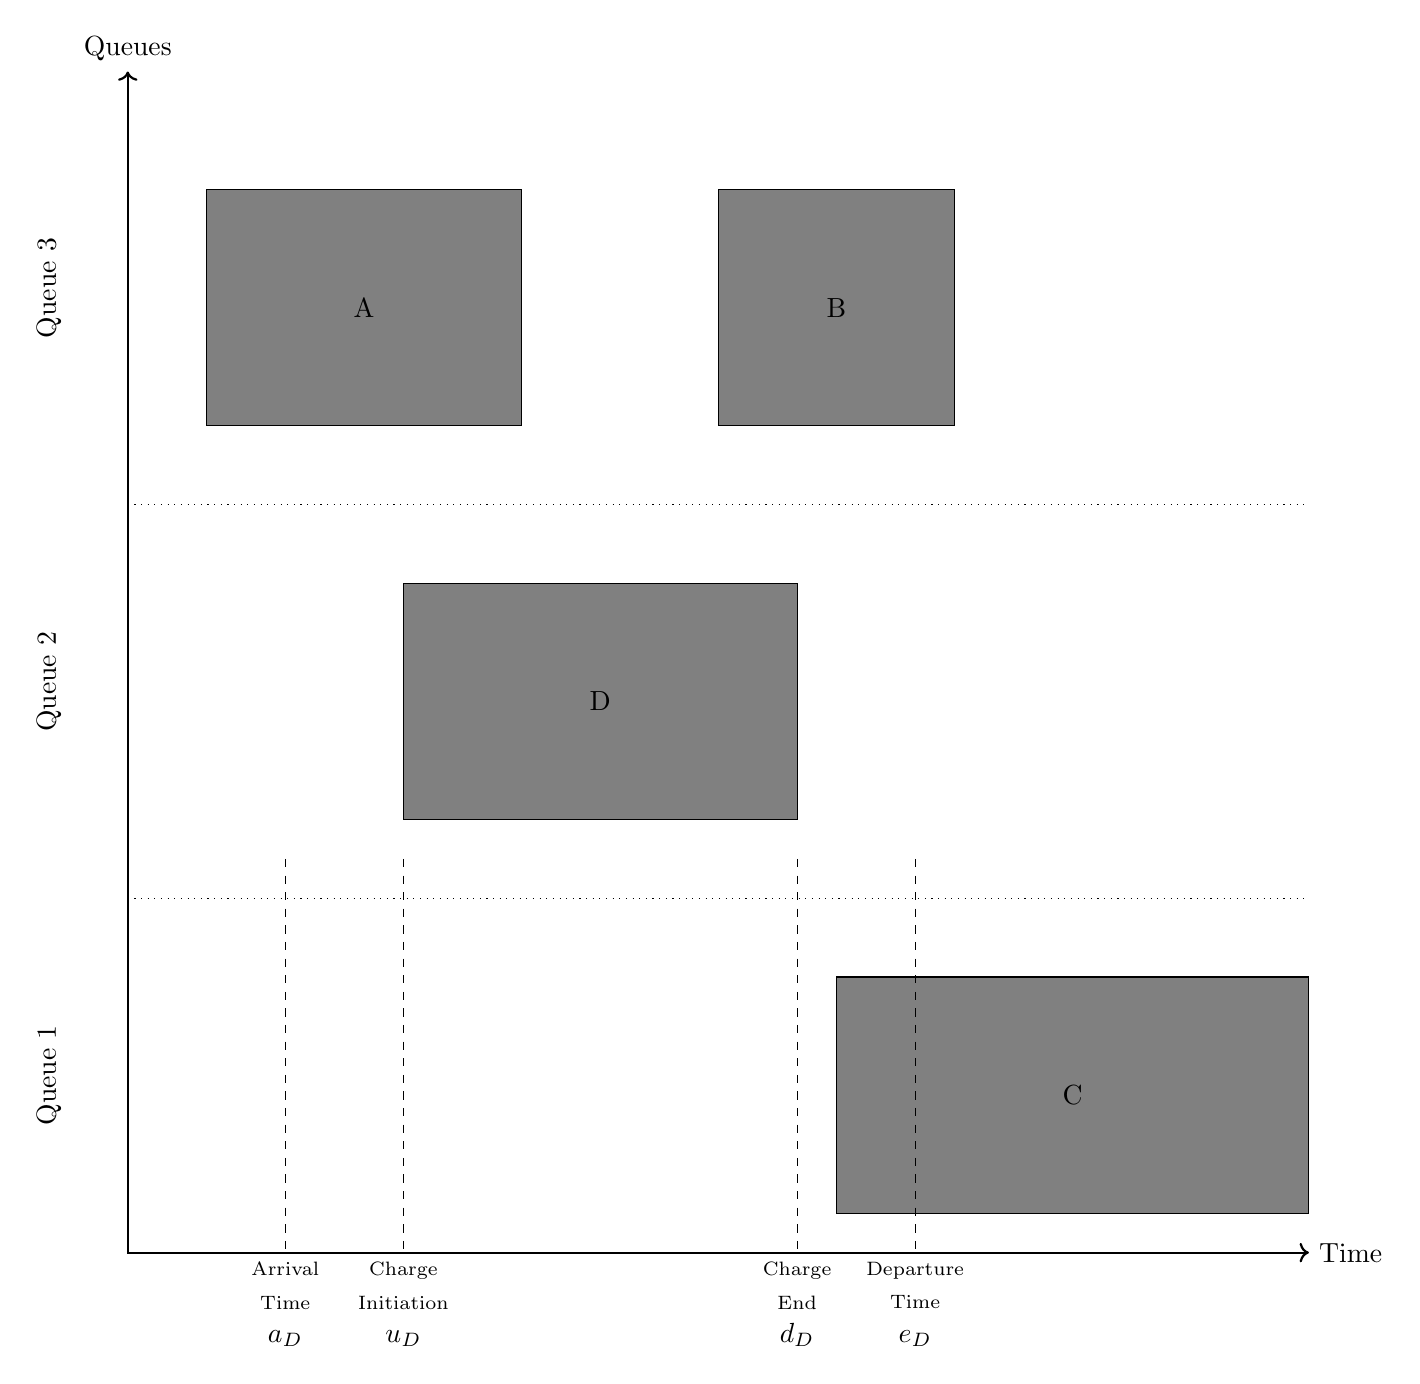
\begin{tikzpicture}
      % Variables
      \def \arrx   {2.0}
      \def \initx  {3.5}
      \def \endx   {8.5}
      \def \depx   {10.0}
      \def \yshift {5}

      % Axis
      \draw [thick,<->] (0,15) node[above]{Queues} -- (0,0) -- (15,0) node[right]{Time};

      % Rectangles
      \node[rectangle, draw, fill=gray, minimum width=4cm, minimum height = 3cm] at (3,12) {A};
      \node[rectangle, draw, fill=gray, minimum width=3cm, minimum height = 3cm] at (9,12) {B};
      \node[rectangle, draw, fill=gray, minimum width=5cm, minimum height = 3cm] at (6,7) {D};
      \node[rectangle, draw, fill=gray, minimum width=6cm, minimum height = 3cm] at (12,2) {C};

      % X-axis labels
      \node [below,align=center] at (\arrx,0) {\scriptsize Arrival     \\ \scriptsize Time \\ $a_D$};
      \node [below, align=center] at (\initx,0) {\scriptsize Charge    \\ \scriptsize Initiation  \\ $u_D$};
      \node [below, align=center] at (\endx,0) {\scriptsize Charge     \\ \scriptsize End \\ $d_D$};
      \node [below, align=center] at (\depx,0) {\scriptsize Departure  \\ \scriptsize Time \\ $e_D$};

      % Y-axis labels
      \node[rotate=90] at (-1, 2.25) {Queue 1};
      \node[rotate=90] at (-1, 7.25) {Queue 2};
      \node[rotate=90] at (-1, 12.25) {Queue 3};

      % Vertical lines
      \draw[dashed] (\arrx,\yshift)--(\arrx,0);
      \draw[dashed] (\initx,\yshift)--(\initx,0);
      \draw[dashed] (\endx,\yshift)--(\endx,0);
      \draw[dashed] (\depx,\yshift)--(\depx,0);

      % Horizontal lines
      \draw[dotted] (0, 4.5) -- (15, 4.5);
      \draw[dotted] (0, 9.5) -- (15, 9.5);

    \end{tikzpicture}
  }}
  \caption{The representation of the queue-time space. The x and y-axis represent time and space, respectively. Along the y-axis, the dashed lines represent discrete queuing locations. The shaded rectangles represent schedules BEBs to be charged. The height of each shaded rectangle represents the space taken on the queue and the width being the time to service said BEB. The vertical dashed lines are associated with vessel D and represent the arrival time, initial charge time, charge completion time, and departure time. Note that the arrival time may be before the initial charge time and the completion time may before the departure time.}
  \label{fig:spacial-and-temporal-constr}
\end{figure}

\section{Optimization Problem}
\label{sec:optimization-problem}
The problem outlined in this work is presented in the form of an objective function with MILP constraints. The MILP
constraints ensure that candidate solutions are operationally feasible. The optimization variables are introduced in
\ref{sec:parameter-definitions}. The objective function is broken down into four major components: consumption cost, demand
cost, assignment cost, and under-charging cost (i.e. a penalty for not meeting minimum charge requirements). The
constraints will then be introduced in \ref{sec:constraints}. The objective function is introduced in
\ref{sec:objective-function}.

\subsection{Variable Definitions}
\label{sec:parameter-definitions}
This section defines the input and decision variables used by the system. The input parameters are assumed to be fixed
prior to optimizing the system. The decision variables are the values that the SA algorithm has the freedom to
manipulate. The variables to be introduced are summarized in \ref{tab:variables}.

\subsubsection{Input Parameters}
\label{sec:input-variables}
The parameters are assumed to be known prior to optimization. They will be presented in two sections: battery dynamics
parameters then packing and discretization parameters. The Battery dynamic parameters are those associated with the SOC
of the BEB, the packing and discretization parameters are those that are associated with BEB placement and the method of
discretizing the system.

\paragraph{Battery Dynamic Parameters}
\label{sec:battery-dynamic-parameters}
The amount energy required to complete the bus route after visit \(i\) is denoted as \(\Delta_i\). There are no routes after the
last visit for each BEB; thus; the energy consumed after the final visit is zero. Let the set of final visits for all
BEBs be denoted as \(\Isetfinal\). That is, the cardinality of the set is \(\lvert \Isetfinal \rvert = n_B\) where \(i \in
\Isetfinal \subset \Iset\) specifies the index for the final visit of bus. The discharge for the final visit of each BEB is
then defined as \(\Delta_{i} = 0; \forall i \in \Isetfinal\). The initial SOC percentage of bus \(b\) at the beginning of the working day
is denoted as \(\alpha_b\). Let \(\Isetinit\) denote the set of initial visit indices for each BEB and let \(\Xi_i \in B\) denote the
identification number of the BEB for visit \(i\). The initial SOC for bus \(\Xi_i\) can be represented as \(\eta_{i} =
\alpha_{\Xi_i}\kappa_{\Xi_i}; \forall i \in \Isetinit \subset \Iset\) where \(\kappa_{\Xi_i}\) is the battery capacity for bus \(\Xi_i\). Lastly, \(r_q\) represents
the power supplied from the charger in queue \(q \in Q\).

\paragraph{Packing and Discretization Parameters}
\label{sec:packing-and-discretization-paramaters}
The cost for assigning a charger to queue \(q \in Q\) is defined by \(\epsilon_q\). \(\xi_i\) represents the next arrival index for bus
\(b_i\). In other words, suppose the ID of each BEB is recorded in order of arrival. Further suppose that recorded list is
\(\xi = \{ 2,1,3,2 \}\), using a starting index of 1, \(\xi_1 = 4\) as that is the next visit by bus 2. The arrival and
departure times of bus visit \(i\) to the station are denoted as \(a_i\) and \(e_i\), respectively. The notation \(t_h\) is used
to denote a discrete time that is employed to calculate the demand cost. \(dt_h\) is the discrete time step \(dt_h = t_h -
t_{h-1}\).

\begin{table}[htbp]
\caption{\label{tab:variables}Table of variables used in the paper.}
\centering
\begin{tabularx}{\textwidth}{L{0.3} L{1.2} L{0.3} L{1.2}}
\textbf{Variable} & \textbf{Description} & \textbf{Variable} & \textbf{Description}\\[0pt]
\hline
Constants &  & Constants & \\[0pt]
\(D\) & Penalty method gain factor & \(n_B\) & Number of buses in use\\[0pt]
\(\T\) & Time horizon & \(n_K\) & Number of iterations in the repetition schedule\\[0pt]
\(n_M\) & Total number of steps created by initial temperature, \(\Tau_0\), and cooling schedule & \(n_Q\) & Number of chargers\\[0pt]
\(n_V\) & Total number of visits & \(n_h\) & Number of discrete steps in time horizon\\[0pt]
\hline
Input variables &  & Input Variables & \\[0pt]
\(\Delta_i\) & Discharge of visit over after visit \(i\) & \(\alpha_b\) & Initial charge percentage time for bus \(b\)\\[0pt]
\(\epsilon_q\) & Cost of using charger \(q\) & \(\kappa_b\) & Battery capacity for each BEB\\[0pt]
\(\rho_i\) & Duration for route after visit \(i\) & \(\xi_i\) & The next index bus \(b\) will arrive\\[0pt]
\(a_i\) & Arrival time of visit \(i\) & \(\Xi_i\) & ID for bus visit \(i\)\\[0pt]
\(t_h\) & Discrete step in time horizon & \(dt_h\) & Discrete time slice in time horizon \(dt_h = t_h - t_{h-1}\)\\[0pt]
\(k\) & Local search iteration \(k\) & \(e_i\) & Time bus visit \(i\) must exit the station\\[0pt]
\(r_q\) & Charge rate of charger \(q\) & \(t_m\) & Element of the temperature vector created by temperature function, \(t_m \in t\)\\[0pt]
\(\nu_b\) & Minimum charge percentage allowed for each BEB &  & \\[0pt]
\hline
Direct Decision Variables &  & Direct Decision Variables & \\[0pt]
\(u_i\) & Initial charge time for visit \(i\) & \(d_i\) & Final charge time for charger for visit \(i\)\\[0pt]
\(q_i\) & Assigned queue for visit \(i\) &  & \\[0pt]
Indirect Decision Variables &  & Indirect Decision Variables & \\[0pt]
\(\eta_i\) & Charge for the bus upon arrival visit \(i\) & \(s_i\) & Amount of time spent on charger for visit \(i\)\\[0pt]
\(\sigma_{ij}\) & Binary variable determining temporal ordering of vehicles \(i\) and \(j\) & \(\psi_{ij}\) & Binary variable determining spatial ordering of vehicles \(i\) and \(j\)\\[0pt]
\(p_{d}\) & Demand cost of the schedule & \(\phi_i\) & Penalty method for visit \(i\)\\[0pt]
\(\C\) & Set of available charging times &  & \\[0pt]
\hline
\end{tabularx}
\end{table}

\subsubsection{Decision Variables}
\label{sec:decision-variables}
Decision variables are those chosen by the optimizer. The variables will be broken into two sections: direct and slack
variables. Direct decision variables are those that the system manipulates directly, and slack variables are those that
are functions of the direct.

\paragraph{Direct Decision Variables}
\label{sec:direct-decision-variables}
The first two variables are \(u_i\) and \(d_i \; \forall i \in \Iset\). They represent the initial and final charging times. These
values must remain within range of the arrival and departure times, \([a_i, e_i]\), for visit \(i\). The last direct
decision variable is the queue that bus visit \(i\) can be placed in to charge, \(q_i \in \Qset\).

\paragraph{Slack Variables}
\label{sec:slack-decision-variables}
Let the initial SOC for a visit be written as \(\eta_i\), where \(i \in \Iset \setminus \Iset_0\). The initial charge for visit \(i\) forms
the foundation from which the SOC of the next visit, \(\eta_{\xi_i}\), is calculated. The charge for bus \(i\)'s next visit is
equal to the initial charge for visit \(i\) plus the charge added to it by charger \(q_i\) over duration \(s_i = d_i - u_i\)
minus the discharge accumulated over route \(i\), i.e.

\begin{equation}
\label{eq:bat-chain}
  \eta_{\xi_i} = \eta_i + r_{q_i}s_i - \Delta_i\text{.}
\end{equation}

The variables \(\sigma_{ij}\) and \(\psi_{ij}\) are used to indicate whether a visit pair \((i, j)\) overlap the same space, as show
in \ref{fig:overlap}. These spatiotemporal variables uphold the following relationships:

\begin{subequations}
\label{eq:bus-spat-temp}
\begin{equation}
  \sigma_{ij} =
  \begin{cases}
    1 & \text{if } u_j \ge d_i, \; i \ne j\\
    0 & \text{otherwise}
  \end{cases}
\end{equation}

\begin{equation}
  \psi_{ij} =
  \begin{cases}
    1 & \text{if } q_j \ge q_i,\; i \ne j\\
    0 & \text{otherwise}
  \end{cases}
\end{equation}
\end{subequations}

That is, for every visit, \(\sigma_{ij} = 1 \implies\) the start charge time of visit \(j\) is greater than the end charge time
of visit \(i\). Similarly, \(\psi_{ij} = 1 \implies\) the queue for visit \(j\) is of a greater index than visit \(i\).

The variable \(\C\) is the set that describes the availability for all chargers. That is, \(\C\) is a set of \(n_Q\) sets that
contain available charger times for each queue \(q \in Q\). Let a set of available charge times for queue \(q\) be defined as
\(\C_q\).

\subsection{Objective Function}
\label{sec:objective-function}
This work aims to minimize the total ``cost'' of utilizing a given charge schedule. Let \(J(\I)\) represent the objective
function. The objective function for this problem has four main considerations: charger assignment, consumption cost,
demand cost, and penalty for an insufficient initial SOC. Each of which will be discussed in turn in the subsequent
sections.

\subsubsection{Assignment Cost}
\label{sec:assignment-cost}
The assignment cost represents the costs of assigning a bus to a particular queue. This is done as a method of
minimizing the total utilized chargers. The assignment cost is written as

\begin{equation}
\label{eq:assignment-cost}
\sum_{i=1}^{n_V} \epsilon_{q_i}r_{q_i}\text{.}
\end{equation}

This cost is effectively the cost on the choice of \(q\). Recalling the form of \(Q\), particularly the ordering in which
the set was defined. Taking \(\epsilon\) to be constructed using the same ordering (idle, slow, then fast charging queues), let
the first \(n_B\) queues have no cost. Furthermore, let the next \(n_Q\) charging queues be of the form \([P, 2P, ...,
n_QP]\). Concatenating these vectors yields \(\epsilon = [[0; n_B], [P, 2P, ..., Pn_Q]]\), where \([0; n_B]\) is used to denote a
vector populated with zeros of length \(n_B\). In words, this form accrues no cost when assigning a BEB to an idle queue
while still minimizing charger count and encouraging the use of slow chargers over fast. Thus, the larger the index of
\(q\), the larger the cost. The \(\epsilon\) vector described above is one of many forms that the vector may take; however, form
shown described is what is applied in this work.

\subsubsection{Penalty Method}
\label{sec:penalty-method}
A penalty method is to be implemented in the objective function that is enabled when the \(\eta_i\) falls below a defined
threshold. Let the piecewise function that enables/disables the penalty method be of the form

\begin{equation}
\label{eq:penalty}
  \phi(x) =
  \begin{cases}
    0   & x \ge 0 \\
    x^2 & x < 0\\
  \end{cases}
\end{equation}

Furthermore, letting \(x = \eta_i - \nu_{\Xi_i} \kappa_{\Xi_i}\), where \(\nu_{\Xi_i} \kappa_{\Xi_i}\) is the minimum charge threshold, applies a penalty
proportional to the difference of the SOC and the threshold squared.

\begin{figure}[htpb]
  \centering \includegraphics{img/overlap}
  \caption{Examples of different methods of overlapping. Space overlap: $q_{k_1} > q_{i} + 1 \therefore \psi_{ik_{1}} = 1$.
    Time overlap $u_{k_2} < u_{j} + s_j \therefore \sigma_{k_{2}j} = 0$. Similarly, $\sigma_{k_3 i} = 0$.}
  \label{fig:overlap}
\end{figure}

Using the form of \ref{eq:penalty} with and added scalar, \(D\), is employed so that the cost of deviating from the threshold
heavily influences the outcome of the objective function. Therefore, the penalty method is written as

\begin{equation}
\label{eq:penalty-method}
\sum_{i=1}^{n_V} D \phi_i(\eta_i - \nu_{\Xi_i} \kappa_{\Xi_i})\text{.}
\end{equation}

\subsubsection{Consumption Cost}
\label{sec:consumpction-cost}
In most cases, energy companies rely on a volumetric rate as a method of track customer electricity consumption (i.e.
total electricity consumed over a billing period). As such, a method of reducing the total energy consumed by the system
is desired. The energy total energy consumed by a charge schedule is defied by what is known as the consumption cost.
The consumption cost is the summation of all the energy being used over all the active periods for each charger in the
time horizon. This is represented by the summation

\begin{equation}
\label{eq:consumption-cost}
\sum_{i=1}^{n_V} r_{q_i}s_i\text{.}
\end{equation}

That is, the charge rate, \(r_{q_i}\), for the active charger, \(q_i\), is multiplied by the time that the charger will be
utilized, \(s_i\).

\subsubsection{Demand Cost}
\label{sec:demand-cost}
Historically for large industrial customers, energy companies often further rely on a demand cost in conjunction with a
consumption cost for billing. The consumption cost is an important metric as it measures how much power a customer may
require over billing period. Energy companies, having to potentially meet large peaks in demand, offset that cost to the
customer. Thus, when a demand and consumption costs are imposed, not only is the total energy reduction desirable, but
also how much power is consumed at a given moment.

A method of calculating the demand charge is done by calculating the average power consumption over a given period of
time. Let the average power used over an arbitrary interval, \(T_p\), be represented by

\begin{equation}
\label{eq:p}
p_{T_p}(t) = \frac{1}{T_p} \int_{t-T_p}^{t} p(\tau) d\tau\text{.}
\end{equation}

Energy companies take the largest peak when calculating the demand cost. Therefore, let the cost of the peak power
consumption be dictated by the maximum average power:

\begin{equation}
\label{eq:pmax}
p_{max}(t) = \max\limits_{\tau \in [0,t]}p_{T_p}(\tau)\text{.}
\end{equation}

Furthermore, a fixed minimum average power is introduced that is intended to act as a base threshold before the cost
begins to increase. Let this fixed threshold be defined as \(p_{fix}\), the demand cost is calculated using

\begin{equation}
\label{eq:pdem}
p_d(t) = \max(p_{fix},p_{max}(t))\text{.}
\end{equation}

Hence, \ref{eq:pdem} defines a cost beginning with a value of \(p_{fix}\) from which it may only increase if \(p_{15}(t) >
p_{fix}\).

Although the charge times for each BEB is continuous, due to the discrete nature of visits it is simpler to determine a
vector of discrete power consumption over the time horizon from which the average power demand cost may be derived. To
discritize \(p_d\), let \(h \in \{ 1, 2, ..., n_H \} \subset \mathcal{Z}\) where \(n_H\) is the total number of steps. Furthermore, let \(p\)
define the vector of discrete power consumption over some time interval and let \(p_h \in p\) be the discrete power demand
at time step \(h\). For conciseness of notation \(t_h\) will be abused to denote the time in discrete form (as opposed to
\(t\) being continuous), let \(dt_h = t_h - t_{h-1}\), and \(\Hset = \{ 1, 2, ..., n_H \}\). Thus, for a given visit \(i\), the
corresponding discrete indices of \(h \in \Hset\) for the range \([u_i, d_i]\) can be determined by first calculating the
total number of steps, \(n_h = \frac{d_i - u_i}{dt}\). Once the number of steps is known, the consumed power, \(r_{vi}\) can
be added to the correct indices in \(p\).

To derive \(p\), a vector of discrete power consumption over the time horizon, utilizing scheduled visits is outlined in
\ref{alg:calc-p}. In other words, the objective of \ref{alg:calc-p} to calculate a vector, \(p\), that defines the power
consumed over discrete steps throughout time horizon. Line 2 defines the time over which the average power will be
calculated. Line 3 initializes a vector, \(p\), with \(n_H\) elements populated with zeros. The vector \(p\) is used to store
the power consumption for each discrete step over the time horizon \(\T\). Line 5 calculates the number of elements in the
charge time \(s_i\). Line 6 calculates the index of \(p\) for all \(n_h\) steps and iterates through each index. Line 7 adds
the power consumed by charging \(q_i\) for the \(h^{\text{th}}\) step.

\begin{algorithm}[H]
  \scriptsize
  \caption{Calculate vector of power cosumption, $p$, by discretizing a charge time frame, $[u_i, d_i]$, into $n_h$ steps and calculating the appropriate index $h \in \{1,2,...,n_H\}$.} \label{alg:calc-p}
  \LinesNumbered
  \TitleOfAlgo{Calculate $p$}
  \KwIn{$(\I, r)$}
  \KwOut{$p$}

  \Begin
    {
      $dt \leftarrow \frac{\T}{n_H}$\tcc*{Calculate the step size}
      $p \leftarrow [0.0; n_H]$\tcc*{Allocate an $n_H \times 1$ vector filled with zeros}

      \tcc{For each visit}
      \ForEach {$\I_i \in \I$}
      {
        $n_h \leftarrow \frac{\I_{i.d} - \I_{i.u}}{dt}$\tcc*{Calculate the total number of steps in the time slice}

        \tcc{For each index in the time slice $[u_i, d_i]$}
        \ForEach {$h \in \{\frac{u_i}{dt}, \frac{u_i + dt}{dt}, ..., \frac{u_i + n_h dt}{dt}\}$}
        {
          $p[h] \leftarrow p[h] + r_{\I_{i.q}}$\tcc*{Add the consumed power during discrete step}
        }
      }
      \Return{$p$}
    }
\end{algorithm}

With the consumed power calculated for each time step, the average power consumption for each interval in the time
horizon can be written as follows:

\begin{equation}
p_{T_p}[h] = \frac{1}{T_p} \sum_{h-\frac{T_p}{dt}+1}^h p_h,
\end{equation}

where \(T_p \le h \le n_H\). Similarly to before, the maximum \(p_{T_p}[h]\) value is to be retained via \(p_{max} =
\max\limits_{h \in H}p_{T_p}[h]\). Thus, the discrete demand cost is expressed as

\begin{equation}
\label{eq:pd-dis}
  p_d = \max(p_{fix}, p_{max})z\text{.}
\end{equation}

To conclude this section, the objective function is to written in its entirety:

\begin{equation}
\label{eq:objective-function}
  J(\I) = p_d + \sum_{i=1}^{n_V} \epsilon_{q_i}r_{q_i} + D \phi_i(\eta_i - \nu_{\Xi_i} \kappa_{\Xi_i}) + r_{q_i}s_i\text{.}
\end{equation}

\subsection{Constraints}
\label{sec:constraints}
While the objectives are used to compare solutions, constraints are introduced to ensure that the solutions are
operationally valid. Operationally validity requires that allocated BEBs do not overlap spatially or temporally.
Furthermore, the SOC of a bus at a particular visit is related to the charge its previous visit by the amount of
charging and discharging that has occurred. Finally, buses must leave the charger before their scheduled departure time.
These constraints are represented as follows:

\begin{multicols}{2}
\begin{subequations}
\label{eq:constraints}

  \begin{equation}
      \label{seq:c0}
      u_j - d_i - (\sigma_{ij} - 1)T \ge 0
  \end{equation}
  \begin{equation}
      \label{seq:c1}
      q_j - q_i - 1 - (\psi_{ij} - 1)Q \ge 0
  \end{equation}
  \begin{equation}
      \label{seq:c2}
      \sigma_{ij} + \sigma_{ji} \le 1
  \end{equation}
  \begin{equation}
     \label{seq:c3}
      \psi_{ij} + \psi_{ji} \le 1
  \end{equation}
  \begin{equation}
      \label{seq:c4}
      \sigma_{ij} + \sigma_{ji} + \psi_{ij} + \psi_{ji} \ge 1
  \end{equation}
  \begin{equation}
      \label{seq:c5}
      s_i = d_i - u_i
  \end{equation}
  \begin{equation}
      \label{seq:c6}
       \eta_{\xi_i} = \eta_{i} + r_{q_i}s_i - \Delta_i
  \end{equation}
  \begin{equation}
      \label{seq:c7}
      \kappa_{\Xi_i} \geq \eta_{i} + r_{q_i}s_i
  \end{equation}
  \begin{equation}
      \label{seq:c8}
      a_i \leq u_i \leq d_i \le e_i \le \T
  \end{equation}
\end{subequations}
\end{multicols}

Constraints \ref{seq:c0}-\ref{seq:c4} are the ``queuing constraints''. They prevent overlap both spatially and temporally
as shown in \ref{fig:overlap}. The y-axis represents the possible queues for a bus visit to be placed into, and the
x-axis represents the time that can be reserved for each visit. The shaded rectangles represent time that has been
scheduled in the horizontal direction, and the queue allocated for each bus visit in the vertical direction. In other
words, the set of constraints \ref{seq:c0} - \ref{seq:c4} aim to ensure that these shaded rectangles never overlap.

Constraint \ref{seq:c0} states that the starting charge time for BEB \(u_j\) must begin after the previous BEB departs,
\(d_i\). The constraint utilizes big-M notation to activate or deactivate the constraint. A value of \(\sigma_{ij} = 1 \implies\)
bus \(i\) has detached from the charger before bus \(j\) has begun charging. If \(\sigma_{ij} = 0\), then the constraint is of the
form \(\T + d_i > u_j\) rendering the constraint ``inactive'' because \(u_j\) cannot be larger than \(\T + d_i\). Similarly, for
\ref{seq:c1}, \(\psi_{ij}\) determines whether the vehicles are charging in the same queue. A value of \(\psi_{ij} = 1 \implies\)
BEB \(i\) is in a queue index that is less than BEB \(j\). If \(\psi_{ij} = 0\) then the constraint is deactivated. Constraints
\ref{seq:c2} - \ref{seq:c4} enforce spatial and temporal ordering between each queue/vehicle pair. \ref{seq:c2} and
\ref{seq:c3} ensure that BEB \(i\) is not placed before and after \(j\) spatially, temporally, or both because that is
impossible. \ref{seq:c4} ensures that BEB \(i\) and \(j\) do not have scheduling conflicts spatially or temporally.

 \ref{seq:c5} describes the service time of the bus. \ref{seq:c6} calculates the initial charge for the next visit for
bus \(b_i\). \ref{seq:c7} ensures that the bus is not being over-charged. \ref{seq:c8} ensures the continuity of the times
(i.e. the arrival time is less than the initial charge which is less than the detach time which is less than the time
the bus exits the station and all must be less than the time horizon).

\section{Simulated Annealing}
\label{sec:simulated-annealing}
SA is a well-studied local search metaheuristic used to solve various optimization problems
\cite{gendreau-2018-handb-metah,press-1992-numer-recip}. A metaheuristic is a high-level problem-independent algorithm
framework that provides a set of guidelines or strategies to develop heuristic optimization algorithms
\cite{radosavljevic-2018-metah-optim}. That is, metaheuristic strategies provides guidelines for implementation;
however, each problem must tailor its implementation to meet its particular needs.

SA is an exploitation oriented, single-solution based metaheuristic. In addition to the advantages of simplicity, both
theoretically and in its implementation \cite{gendreau-2018-handb-metah,radosavljevic-2018-metah-optim}. SA is also of
considerable interest for global optimization over regions containing several local and global minima due to inherent
non-linearities of the objective function \cite{gendreau-2018-handb-metah}. This model is named after its analogized
process where a crystalline solid is heated then allowed to cool at a slow rate until it achieves its most regular
possible crystal lattice configuration (i.e. its minimum lattice energy state)
\cite{henderson-1989-theor-pract,press-1992-numer-recip}. SA establishes a connection between this thermodynamic
process and the search for global optima in optimization problems.

There are three key components to SA: cooling schedule (temperature function), acceptance criteria, and generation
mechanisms \cite{keller-2019-multi-objec,press-1992-numer-recip}. The temperature function describes the speed at
which the system is ``cooled'' over each iteration. The term ``system'' refers to a general instance of SA. The generation
mechanisms provide a means of modifying the system by some singular discrete change that is within the neighborhood of
the previous solution \cite{gendreau-2018-handb-metah}. The acceptance criteria is a function of the system temperature
that makes the decision whether the system will accept an inferior solution in favor of exploring the solution space.
Finally, the constant temperature iteration count is the number of steps taken to try to exploit a solution at a
constant temperature. Each of these mechanisms are elaborated in the subsequent sections.

\subsection{Cooling Equation}
\label{cooling-equation-experimental}
The temperature function models a ``rate of cooling'' for the SA process. Initially, when the temperature is high, SA
encourages exploration. As the process begins to ``cools down'' (in accordance to the cooling schedule), it begins to
encourage local exploitation of the solution (rather than exploration)
\cite{rutenbar-1989-simul-anneal-algor,henderson-1989-theor-pract}. There are three common basic types of cooling
equations: linear, geometric, and exponential. Geometric cooling schedules are most widely used in practice
\cite{keller-2019-multi-objec}. As such, it will also be employed by this work. It is defined by the difference
equation

\begin{equation}
\label{eq:cool}
t_m = \beta t_{m-1}\text{.}
\end{equation}

The value of \(\beta\) may vary anywhere between the range \([0,1)\). The further \(\beta\) is from 1, the quicker the function
converges to zero. \ref{fig:geometric} demonstrates this principle by plotting the geometric schedule using varying
values of \(\beta\).

\begin{figure}[t!]
  \centering 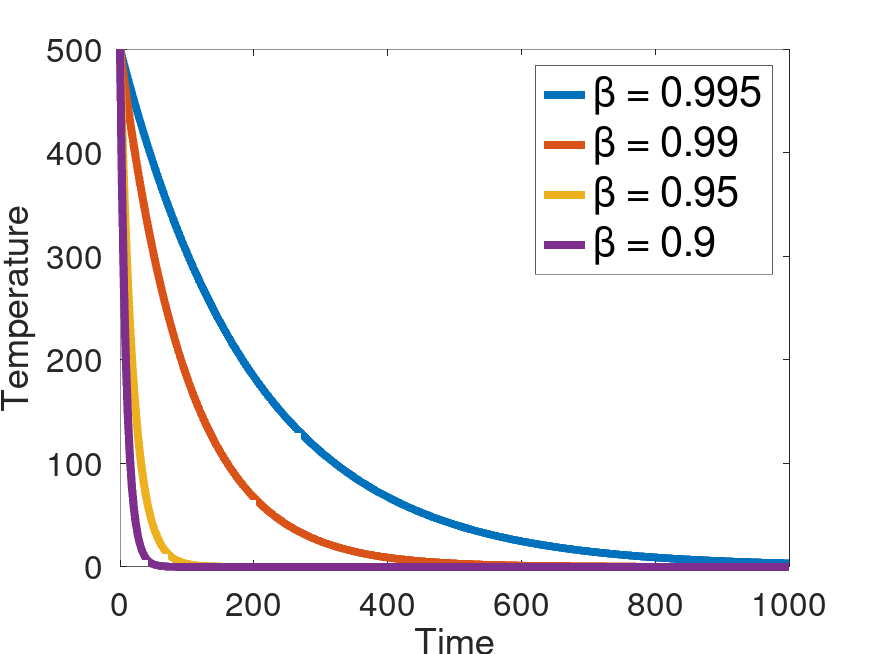
\includegraphics[width=0.6\textwidth]{img/geometric.png}
  \caption{Geometric cooling schedule utilizing various value of $\beta$.}
  \label{fig:geometric}
\end{figure}

\subsection{Acceptance Criteria}
\label{sec:acceptance}
In SA, the algorithm stores a candidate solution that is continuously compared to newly generated solutions. Let the
stored solution be referred to as the ``active solution''. During each iteration, a new candidate solution is generated
and compared to the active solution to determine if the new solution should replace the active solution. To determine if
the active solution is to be replaced, an acceptance criterion is defined. In an effort to encourage exploration,
inferior candidate solutions have a probability of being accepted. The probability of accepting an inferior candidate
solution is described by the function \(\exp(-\frac{J(\I) - J(\bar{\I})}{t_m})\) where \(J(\cdot)\) is the objective function
(\ref{sec:objective-function}), \(t_m\) is current temperature, \(\I\) is the current solution, and \(\bar{\I}\) is the new
candidate solution. Formally, let \(\Delta E \equiv J(\I) - J(\bar{\I})\) and let \(f(\cdot)\) be the function that describes the
probability of accepting a candidate solution \(\bar{\I}\). The probability of accepting a candidate solution is thus of
the form \cite{keller-2019-multi-objec}

\begin{equation}
\label{eq:candaccept}
f(\I,\bar{\I},t_m) =
\begin{cases}
  1                   & \Delta E > 0 \\
  e^{- \frac{\Delta E}{t_m}} & \text{otherwise}
\end{cases}\text{.}
\end{equation}

\subsection{Neighbor Generators and Wrappers}
\label{sec:generation-mechanisms}
Generation mechanisms are used to create a neighboring candidate solution \cite{gendreau-2018-handb-metah}. That is,
the generating function creates a solution that can be reached in a single iteration from the active solution. In the
case of the problem statement made in \ref{sec:problem-description}, five primitive generation mechanism are used: new visit,
slide visit, new charger, new window, wait. The purpose of each of these generators is to assign new visits to a
charger, adjust a bus visits initial and final charge time within the same time frame/queue, move a BEB from one charger
to another with the same charge schedule, move a bus to its idle queue. Each generator will be discussed in more detail
in \ref{sec:generators}.

These generation mechanisms will in turn be utilized by two wrapper functions. The schedule generation is to used create
an initial candidate solutions for SA and the perturb schedule generator is used to take a candidate solution and alter
it slightly in an attempt to step toward a global or local minimum. The wrapper functions will be discussed in
\ref{sec:generator-wrappers}. However, prior to discussing the primitives and wrapper generating functions, their respective
inputs and outputs must be defined.

\subsubsection{Generator Input/Output}
\label{sec:generator-input-output}
This section discusses inputs and outputs of each generator. The input consists of the bus visit index of interest, the
current state of visits, \(\I\), and the current state of the charger availability, \(\C\). The output of each generator
affects a subset of \(\I\) and the updated charger availability \(\C\).

\paragraph{Generator Input}
\label{sec:org1aedbe7}
Each generator accepts a tuple \(\Sol \equiv (i, \I, \C)\) where \(i\) is the visit index being manipulated, \(\I\) is the set of
visits, and \(\C\) is the set that describes the availability for all chargers \(q \in \Qset\).

\paragraph{Generator Output}
\label{sec:org4d27b58}
The output of the generating functions is the same as the input, but with changes applied to it by a generator. Let a
modified variable be denoted with a bar, \(\bar{\cdot}\). Thus, the modified input tuple is written as \(\bar{\Sol}\). Although
not all the variables in \(\Sol\) are modified, it is written in this manner for the sake of consistency and simplicity in
bookkeeping.

\subsubsection{Generators}
\label{sec:generators}
This section describes and outlines the different generator types. Recall that to satisfy constraints, \(n_B\) extra idle
queues are added that provide no power to the BEB. Because of this, the set of queues is fully defined where \(Q\) is the
ordered set of idle queues, slow queues, then fast queue. The use case for the idle queues are for when a bus is not to
be placed on a charger. Rather, it will be placed in the queue, \(q \in B\), which satisfies the previously defined spatial
constraints while allowing the bus to be ``set aside''. The charge queues are denoted by \(q \in Q \setminus B\).

In the development of the algorithms, the dot notation is to be introduced to extract variables from tuples. For
example, suppose the arrival time is desired to be extracted from visit \(i\). Given \(\I\), the notation that describes
extracting the initial charge time for visit \(i\) is written as \(u_i \equiv \I_{i.u}\).

\paragraph{New visit}
\label{sec:new-visit}
The new visit generator defined in \ref{alg:new-visit} describes the process of moving a BEB, \(b \in B\), from a waiting
queue, \(q \in B\), to a charging queue, \(q_i \in Q \setminus B\), within its arrival/departure time \([a, e]\). Let \(\U_{\{\cdot\}}\)
indicate that an element is selected randomly with a uniform distribution from the set \(\{\cdot\}\). For example, \(\U_{[a,
e]}\) indicates that a value will be selected between \(a\) and \(e\) with a uniform distribution. \ref{alg:new-visit} begins
by extracting variables. Lines 6 and 7 randomly select a charging queue and available time frame with a uniform
distribution, respectively. Line 8 attempts to assign the visit the time frame found in Line 7, if it succeeds, the
updated visit is returned. Otherwise, the null value is returned.

The function \texttt{findFreeTime} is the algorithm that determines whether a visit's time at the station \([a, e]\) can be placed
in the time availability of charger \(q\). Let the available time for charger \(q\) for visit \(i\) be denoted as \(C \equiv
\C_{i.q}\). Furthermore, let the lower and upper bound of \(\C\) be denoted as \(\C_L\) and \(C_U\), respectively. The
algorithm checks whether the BEB time at the station, \([a_i, e_i]\) fits within the charger availability \([C_L, C_U]\). If
it does, a random charge time slice is returned, otherwise the null value is returned.

\begin{algorithm}[H]
  \scriptsize
  \caption{New visit algorithm}
  \label{alg:new-visit}
  \LinesNumbered
  \TitleOfAlgo{New Visit}
  \KwIn{$\Sol$}
  \KwOut{$\bar{\Sol}$}

  \SetKwFunction{Union}{Union}
  \SetKwFunction{findFreeTime}{findFreeTime}

  \Begin
    {
      $i \leftarrow \Sol_{i}$\tcc*{Extract visit index}
      $a \leftarrow \I_{i.a}$\tcc*{Extract the arrivial time for visit $i$}
      $e \leftarrow \I_{i.e}$\tcc*{Extract the departure time for visit $i$}
      $q \leftarrow \I_{i.q}$\tcc*{Extract the current charge queue for visit $i$}
      $\bar{q} \leftarrow \mathcal{U}_{Q}$\tcc*{Select a random charging queue with a uniform distribution}
      $C \leftarrow \mathcal{U}_{\C_q}$\tcc*{Select a random time slice from $\C_q$}

      \If(\tcc*[f]{If there is time available in $C_q^j$}){($\bar{C}, \bar{u}, \bar{d}$) $\leftarrow$ \findFreeTime{$C, i, q, a, e$} $\not\in \varnothing$}
         {
           \Return{($i, (\bar{q},\bar{u},\bar{d}),\bar{C}$)}\tcc*[f]{Return visit}
         }

         \Return{($\varnothing$)}\tcc*{Return nothing}
    }
\end{algorithm}

\paragraph{Slide visit}
\label{slide-visit}
This primitive generator is used for visits that have already been scheduled. Because of the constraint \ref{seq:c8}
there may be some slack to manipulate \([u_i, d_i]\) within the window \([a_i, e_i]\). That is, two new values, \(u_i\) and
\(d_i\) are randomly selected with a uniform distribution that satisfy the constraint \(a_i \leq u_i \leq d_i \leq e_i\). Line 2 of
\ref{alg:slide-visit} purges the visit from the charger availability schedule. The \texttt{Purge} function simply removes an
assigned charge time from the set \(\C\). Without altering selected queue, the charge time randomly re-assigned with a
uniform distribution. Upon success, the updated tuple is returned, otherwise the null value is returned.

\begin{algorithm}[H]
  \scriptsize
  \caption{Slide Visit Algorithm} \label{alg:slide-visit}
  \LinesNumbered
  \TitleOfAlgo{Slide Visit}
  \KwIn{$\Sol$}
  \KwOut{$\bar{\Sol}$}

    \SetKwFunction{Purge}{Purge}

    \Begin
    {
      $(i, \I, \bar{\C}) \leftarrow$\Purge{$\Sol$}\tcc*{Purge visit $i$ from charger availibility matrix}
      $C \leftarrow \bar{C}_{i.q_i}$\tcc*{Get the time availability of the purged visit}

      \tcc{If there is time available in $C$}
      \If{($\bar{C}, \bar{u}, \bar{d}$) $\leftarrow$ \findFreeTime{$C$, $\Sol_i$, $\I_q$, $\I_{i.a}, \I_{i.e}$} $\not\in \varnothing$}
      {
        \Return{($i, \I, (\I_{i.q_i},\bar{u},\bar{d}),\bar{C}$)}\tcc*[f]{Return updated visit}
      }

        \Return{($\varnothing$)}\tcc*{Return nothing}
    }
  \end{algorithm}

\paragraph{New charger}
\label{new-charger}
The new charger generator moves a visit \(\I_i\) to a new charging queue while maintaining the same charge time, \([u_i,
d_i]\). \ref{alg:new-charger} initial purges the visit from the charger availability set, a queue is selected at random
with a uniform distribution, then the new selection is checked whether the charge time \([u_i, d_i]\) may be assigned to
the new queue.

\begin{algorithm}[H]
  \scriptsize
  \caption{New Charger Algorithm} \label{alg:new-charger} \LinesNumbered \TitleOfAlgo{New Charger} \KwIn{$\Sol$}
  \KwOut{$\bar{\Sol}$}

    \SetKwFunction{Purge}{Purge}

    \Begin
    {
      $(i, \I, \bar{\C}) \leftarrow$\Purge{$\Sol$}\tcc*{Purge visit $i$ from charger availibility matrix}
      $q \leftarrow \mathcal{U}_{Q}$\tcc*{Select a random charging queue with a uniform distribution}

      \If(\tcc*[f]{If there is time available in $C_{q}$}){($\bar{C}, \bar{u}, \bar{d}$) $\leftarrow$ \findFreeTime{$\bar{\C}_{i.q}$, $\Sol_i$, $\I_q$, $\I_{i.a}, \I_{i.e}$} $\not\in \varnothing$}
      {
        \tcc{Return visit, note $u$ and $d$ are the original inital/final charge times.}
        \Return{($i, \I, (q,\I_{i.u}, \I_{i.d}),\bar{\C}$)}
      }

      \Return{($\varnothing$)}\tcc*{Return nothing}
    }
  \end{algorithm}

\paragraph{Wait}
\label{sec:wait}
The wait generator simply removes a bus from a charger queue and places it in its idle queue, \(q_i \in B\). \ref{alg:wait}
begins by purging the visit from the charger availability set, the visit is then assigned to its idle queue for the
duration of its time at the station.

\begin{algorithm}[H]
\scriptsize
\caption{Wait algorithm} \label{alg:wait}
    \LinesNumbered
    \TitleOfAlgo{Wait}
    \KwIn{$\Sol$}
    \KwOut{$\bar{\Sol}$}

    \SetKwFunction{Purge}{Purge}

    \Begin
    {
      $(i, \I, \bar{\C}) \leftarrow$\Purge{$\Sol$}\tcc*{Purge visit $i$ from charger availibility matrix}
      $\bar{\C}'_{\I_{i.\Gamma_i}} \leftarrow \C' \cup \{[\I_{i.a}, \I_{i.e}]\}$\tcc*{Update the charger availability matrix for wait queue $\bar{\C}_{i.q_i}$}
      \Return{$(i, \I, (\I_{i.b}, \I_{i.a}, \I_{i.e}), \bar{\C})$}\tcc*[f]{Return visit}
    }
  \end{algorithm}

\paragraph{New Window}
\label{sec:new-window}
New window, as shown in \ref{alg:new-window}, is a combination of \ref{alg:new-visit} (new visit) and \ref{alg:wait}
(wait). By this it is meant that visit \(i\) is placed in its wait queue then added back in as if it were a new visit.
This implies that the BEB may be assigned to a different queue and a new charge time slice. \ref{alg:new-window} begins
by purging the visit from the charger availability set. \ref{alg:wait} is executed, upon success, \ref{alg:new-visit} is
executed. If that succeeds, return the updated tuple, otherwise return the null value.

\begin{algorithm}[H]
  \scriptsize
  \caption{New window algorithm} \label{alg:new-window}
  \LinesNumbered
  \TitleOfAlgo{New Window}
  \KwIn{$\Sol$}
  \KwOut{$\bar{\Sol}$}

  \SetKwFunction{NewVisit}{NewVisit}
  \SetKwFunction{Wait}{Wait}

  \Begin
  {
    $\bar{\Sol} \leftarrow$\Wait{$\Sol$}\tcc*{Assign visit to its respective idle queue}
    \If(\tcc*[f]{Add visit $i$ back in randomly})
       {
         $\bar{\bar{\Sol}} \leftarrow$ \NewVisit{$\bar{\Sol}$} $\not\in \varnothing$
       }
       {
         \Return{$\bar{\bar{\Sol}}$} \tcc*[f]{Return visit}
       }

       \Return{($\varnothing$)}\tcc*{Return nothing}
  }
\end{algorithm}

\subsubsection{Generator Wrappers}
\label{sec:generator-wrappers}
This section covers the algorithms utilized to select and execute different generation processes. The generator wrappers
are the methods immediately called by the SA algorithm. Each wrapper utilizes the primitive generators previously
described and returns either a new charge schedule or a modified charge schedule.

\paragraph{Charge Schedule Generation}
\label{sec:charge-schedule-generation}
The objective of \ref{alg:charge-schedule-generation} is to assign each visit to a random charge queue and charge time.
Specifically, this generator exists to initialize the system with a solution in a greedy manner.
\ref{alg:charge-schedule-generation} loops through each visit and executes \ref{alg:new-visit} to place visit \(i\) at
random queue with a random charge time.

\begin{algorithm}[H]
\scriptsize
\caption{Charge schedule generation algorithm} \label{alg:charge-schedule-generation}
    \LinesNumbered
    \TitleOfAlgo{Candidate Solution Generator}
    \KwIn{$\Sol$}
    \KwOut{$\bar{\Sol}$}

    \SetKwFunction{NewVisit}{NewVisit}

    \Begin
    {
        \tcc{Select an unscheduled BEB visit from a randomly indexed set of visits}
        \ForEach {$\I_i \in \I$}
        {
            ($i, \bar{\I}$, $\bar{\C}$) $\leftarrow$ \NewVisit{($\I_i$, $\I$, $\C$)}\tcc*{Assign the bus to a charger}
        }
            \Return{($0, \bar{\I}$, $\bar{\C}$)}
    }
  \end{algorithm}

\paragraph{Perturb Schedule}
\label{sec:tweak-schedule}
Once the active solution has been created by \ref{alg:charge-schedule-generation}, the SA process begins modifying it to
create candidate solutions. After each step of the cooling function, the active solution will be altered \(n_K\) times by
a random primitive generator. During these \(n_K\) iterations the active solution is modified to create a neighboring
candidate solution. This candidate solution will then be compared against the active solution in the manner discussed in
\ref{sec:acceptance}. \ref{alg:perturb-schedule} describes the method by which the SA algorithm decides how to perturb the
schedule. The method that will be employed generate a neighboring solution is as follows: pick a visit, pick a primitive
generator, and execute said primitive generator once. Let \(\W^y_{[\cdot]}\) denote a random selection with a distribution
specified by a weight vector \(y \in \mathbb{R}\). Thus, \ref{alg:perturb-schedule} is as follows: select a visit with a uniform
distribution, select a primitive with a weighted distribution. Letting \(n_G\) denote the number of primitive generating
functions, the selected primitive with a weighted distribution is denoted as \(\W^y_{[1, n_G]}\). The primitive is then
executed, and the results are returned.

\begin{algorithm}[H]
\scriptsize
\caption{Perturb schedule algorithm} \label{alg:perturb-schedule}

    \LinesNumbered
    \TitleOfAlgo{Perturb Schedule}
    \KwIn{$\Sol$}
    \KwOut{$\bar{\Sol}$}

    \SetKwFunction{PGF}{PGF}

    \Begin
    {
        $\I_i\leftarrow\; \U_{\I}$\tcc*{Randomly select a visit}
        $i \leftarrow\; \I_i$\tcc*{Extract visit index}
        $y \leftarrow [y_1, y_2, ...]$\tcc*{Define the weight of each primitive generator}
        $PGF \leftarrow\; \W^y_{[1,n_G]}$\tcc*{Select one of the generator functions}
        $\bar{\Sol} \leftarrow$ \PGF{($i$, $\I$, $\C$)}\tcc*{Excecute the generator function}
        \Return{($0, \bar{\I}$, $\bar{\C}$)}
    }
\end{algorithm}

\subsection{Alternative Heuristic Implementation}
\label{sec:heuristic-implementation}
As suggested by the works in \cite{Zhang_2010,Xinchao_2011}, applying heuristics to the generating functions can
manipulate the searched neighborhoods in a way that may assist the SA algorithm with convergence. As a test to assist in
minimizing charger utilization, a simple heuristic was applied to \ref{alg:new-visit} and \ref{alg:new-charger} in the
method that they select new charging queues. Suppose rather than selecting a queue at random from \(q \in Q\), the
algorithms randomly select whether to place a BEB in a slow or fast charging queue with a weighted distribution favoring
slow chargers. Once the charger type has been selected, the algorithm will then begin incrementally attempting to place
the BEB in a queue of that type beginning from the smallest index of that charger type. For example, if a BEB has been
selected to be placed in a queue with a slow charger, the algorithm begins by attempting to place the BEB in the charger
queue \(q = n_B + 1\). If it is unable to be placed in that queue, it then attempts to be placed in the next queue \(q =
n_B + 2\). This is done incrementally until all the queues have been exhausted. At the expense of an additional up-front
computation cost, the heuristic will attempt to pack the visit optimally in the spacial sense.

\section{Optimization Algorithm}
\label{sec:optimization-algorithm}
This section combines the generation algorithms and the optimization problem into a single algorithm (\ref{alg:sa-pap}).
While the SA PAP generally is written almost identically to that of the general SA algorithm, the general SA assumes
that the generated candidate solutions are in the solution space of the problem, \(\omega \in S\) where \(S\) is the solution
space. Initialization and the perturbation of a schedule must be verified to ensure that the generated schedule is in
the solution space. Therefore, the objective function and constraints introduced in \ref{sec:constraints} and
\ref{sec:objective-function}, respectively, must be employed to verify that the output of
\ref{alg:charge-schedule-generation} is in the feasible space, \(S\).

As previously stated, the generating functions directly influence the values of the assigned charge queue, charge
initialization time, and charge completion time: \(q_i\), \(u_i\), and \(d_i\), respectively. Having generated those values,
the rest of the decision variables may be derived. Let's begin by reviewing over the packing constraints.
\ref{seq:c0}-\ref{seq:c1} are employed to enable and disable \(\sigma_{ij}\) and \(\psi_{ij}\) and \ref{seq:c2}-\ref{seq:c4} ensure
the validity of the values. \ref{seq:c5} can be directly calculated and \ref{seq:c8} is fully defined.

Changing the focus over to the dynamic constraints, similarly to what was seen with the packing constraints, the battery
dynamic constraints are also fully defined and can be calculated. \ref{seq:c6} is sequentially calculated after a given
schedule has been fully defined. \ref{seq:c7} is evaluated to ensure the BEB is not overcharged. The penalty method
implemented in \ref{sec:objective-function} is set in place to allow the SOC to go below the specified threshold, \(\nu_{\Xi_i}
\kappa_{\Xi_i}\), but punish the solution for doing so. Thus, over time, the candidate solutions will be encouraged toward a
solution that does not activate the penalty method (i.e. is solution is truly feasible).

The SA-PAP algorithm in \ref{alg:sa-pap} will now be outlined. The algorithm begins be creating a temperature schedule
and creating an initial solution. The algorithm then begins to iterate through the temperature schedule (outer loop).
For each iteration of the outer loop, an inner loop is executed \(n_K\) times. During this inner loop, the solution is
modified by a generating function to create a candidate solution. The candidate is solution is then compared with the
active solution, and updated according to the acceptance criteria. These actions are performed until the temperature
function is exhausted.

\begin{algorithm}[H]
  \scriptsize
  \caption{Simulated annealing approach to the position allocation problem} \label{alg:sa-pap}
  \LinesNumbered
  \TitleOfAlgo{SA PAP}
  \KwIn{($\I$ , $\C$)}
  \KwOut{($\bar{\I}$, $\bar{\C}$)}

  \SetKwFunction{Temp}{$\Tau$}
  \SetKwFunction{CSG}{CSG}
  \SetKwFunction{PS}{PS}
  \SetKwFunction{Obj}{J}

  \Begin
    {
      \tcc{Generate vector of temperatures given temperature function $\Tau$ and initial temperature $\Tau_0$}
      $t \leftarrow$ \Temp{$\Tau_0$}

      $\Sol \leftarrow$\CSG{($\I$, $\C$)}\tcc{Generate an initial solution}

      \tcc{For each item in the temperature vector}
      \ForEach{$t_k \in t$}
       {
        \tcc{For each step in the constant temperature repitition counter}
        \ForEach{$k \in \{0, 1, ..., n_K\}$}
        {
          $\bar{\Sol} \leftarrow$ \PS{($\I$, $\C$)} \tcc*{Generate a new solution}
          $\Delta E = $ \Obj{$\bar{\Sol}_{\I}$}  - \Obj{$\Sol_{\I}$} \tcc*{Calculate the difference of fitness scores}

          \If{$\bar{\I} \in S$ and $\Delta E < 0$}{$\Sol \leftarrow \bar{\Sol}$}
          \If{$\bar{\I} \in S$ and $\Delta E \ge 0$}{$\Sol \leftarrow \bar{\Sol}$ with probability $e^{\frac{\Delta E}{t_k}}$}
        } % For k
      }   % For t_k \in t

      \Return{($\I$ , $\bar{\C}$)}
    } % Begin
\end{algorithm}

\section{Example}
\label{sec:example}
An example is now provided to demonstrate the utility of the developed SA charge scheduling technique. In
\ref{sec:beb-scenario} a description of the example scenario is presented followed by a brief introduction of the original
MILP PAP. An alternative heuristic based planning strategy called Qin-Modified, and a heuristic modification to the SA
PAP are also used as comparisons to the SA PAP technique presented in this work. \ref{sec:results} presents the results for
each of planning strategies. The results are also analyzed and discussed.

\subsection{BEB Scenario}
\label{sec:beb-scenario}
The test scenario was run over a time horizon of \(T=24\) hours, with a total of \(n_V = \N\) visits to the station shared
between \(n_B = \A\) buses. Each BEB has a battery capacity of \(\kappa_b =\) \batsize kWh battery that is required to stay above
an SOC of \(\nu_b =\) \mincharge (\fpeval{\batsize * \minchargeD} kWh). Each bus is assumed to begin the working day with \(\alpha
=\) \fpeval{\acharge*100}\% charge (\fpeval{\acharge * \batsize} kWh). Each bus is also assumed have a rate of discharge
of \(\Delta =\) 30 kW. The penalty method employs a gain of \(D = \Cgain\). A total of \(n_C =\) \fpeval{\fast + \slow} chargers
are utilized where \slow of the chargers are slow charging (\slows kW) and \fast are fast charging (\fasts kW). As
previously introduced, to encourage the SA PAP to utilize the fewest number of chargers, the value of \(\epsilon_q\) in the
objective function is \(\forall q \in \{1,2,..., n_B \}; \epsilon_q = 0\) and \(\forall q \in Q \setminus B; \epsilon_q = 100q\). The SA algorithm utilizes the
geometric cooling schedule with an initial temperature of \(T_0 = \tempinit\) with \(\beta_2 = 0.999\), resulting in a total of
\(n_M = \tempcnt\) steps. The demand cost is taken over fifteen minute intervals. Thus let the demand cost be denoted as
the peak-15 with the associated symbol \(p_{15}\). A weight vector of \([3, 3, 2, 1]\) was used to influence the
distribution of selecting the new charger, new window, wait, and slide visit primitives, respectively. The algorithm
also assumes a total of \(n_K = \localcnt\) iterations for the local search at a constant temperature. In total, that
results in \fpeval{\localcnt * \tempcnt} configurations being searched. On average each constant temperature
search took an average of \(\quicklocal\) seconds to complete, resulting in a total runtime of
\fpeval{\quicklocal * \tempcnt} seconds.

\ref{sec:heuristic-implementation} introduced the idea of an alternative heuristic implementation for the SA algorithm. To
distinguish the heuristic implementation from the method derived in \ref{sec:generation-mechanisms}, let this implementation
be referred to as ``heuristic'' implementation and the previous as the ``quick'' implementation. Using the same weights for
selecting randomly selecting the primitive generators, the heuristic approach further implemented a weighted
distribution vector of \([3, 1]\) to decide whether to select a slow or fast charger, respectively. In the heuristic
approach, on average the constant temperature search took a total of \(\heuristiclocal\) seconds to complete, resulting in
a total runtime of \fpeval{\heuristiclocal * \tempcnt} seconds. The heuristic generators were expected to be
slightly slower due to its iterative approach.

One of the methods utilized to compare with the SA PAP is the MILP PAP. This framework is the original MILP
implementation of the PAP derived from \cite{qarebagh-2019-optim-sched}. The inputs to the system are the same as those
discussed above. The MILP PAP does not implement the peak-15 in its objective function. In an attempt to compare the
solution of the MILP with the SA output more directly, a similar solve time of 3600 seconds. The MILP was executed
utilizing the Gurobi MILP solver \cite{gurobi-2021-gurob-optim}.

Another heuristic-based optimization strategy, referred to as Qin-Modified, is also employed as a means of comparison
with the results of the SA PAP. The Qin-Modified algorithm is a based on the threshold strategy of
\cite{qin-2016-numer-analy}. The algorithm has been modified slightly to accommodate the case of multiple charger types
without a heuristic search for the best charger type. The heuristic is based on a set of rules that revolve around the
initial charge of the bus at visit \(i\). There are three different thresholds, low (85\%), medium (90\%), and high (95\%).
Buses below the low threshold are prioritized to fast chargers then are allowed to utilize slow chargers if no fast
chargers are available. Buses between the low and medium threshold prioritize slow chargers first and utilize fast
chargers only if no slow chargers are available. Buses above the medium threshold and below high will only be assigned
to slow chargers. Buses above the high threshold will not be charged. Once a bus has been assigned to a charger, it
remains on the charger for the duration of the time it is at the station, or it reaches 95\% charge, whichever comes
first. Note that UTA uses 70\% to decide that a fast charger is required. The previously described simulations were run
on a machine equipped with an AMD Ryzen 9 5900X 12 - Processor (24 core) at 4.95GHz.


\subsection{Results}
\label{sec:results}
The schedules generated by each of the methods is presented in \ref{fig:schedule}. Rows 0-14 represent slow charging
queues and rows 15-29 represent fast charging queues. The symbols represent the initial charge times, and the horizontal
line with the vertical tick signifies the region of time the charger is active. A qualitative comparison between the
different is the perceived lack of organization of the quick SA technique. Although the assignment cost was set in
place, due to the random nature of the queue assignments the simulation was not able to converge to a well-packed
solution. The heuristic approach was able to more successfully able to pack its schedule similarly to the schedule of
the Qin-Modified and MILP PAP.

On the quantitative side of the minimization/packing discussion, the Qin-Modified schedule utilizes one fast and two
slow chargers as can be seen in \ref{subfig:schedule-qin}. The MILP PAP framework generated a schedule that utilizes
three fast charges and four slow chargers as shown in \ref{subfig:schedule-milp}. The heuristic SA strategy created its
schedule with eight slow charger queues and four fast charging queues as shown in \ref{subfig:schedule-heuristic-sa}.
The quick strategy for the SA algorithm created a schedule utilizing fifteen slow and fast chargers as is demonstrated
in \ref{subfig:schedule-quick-sa}. That is to say, the Qin-Modified schedule was able to most effectively minimize the
charger count followed by the MILP PAP, and the heuristic SA, and the work being the quick SA technique. The MILP
produced a schedule with a three charger gap in the fast queues, where the intermediate queues were never used. The
heuristic SA, while possibly being able to move some assignments to a lower charge queue index, did not contain any gaps
of unused queues. The Qin-Modified utilized the fewest chargers overall, but also suffers a lack of optimality in its
packing of the schedule. Thus, none of the methods were able to fully minimize the packing constraint. Note that the SA
algorithm has no guarantee of optimality; therefore, post-processing could be applied to further minimize the charger
indices.

A table of the mean, maximum instantaneous charger use is shown in \ref{tab:charge-count}. The mean is meant to be a
measure of how many slow/fast chargers are being utilized over the time horizon, on average. The maximum and scheduled
rows represent the total amount of queues the system actually utilized in parallel while the scheduled queues represents
the amount of queues a particular schedule calls for. The Qin-Modified only utilized 2 slow chargers, so the mean is
expected to be low (0.788). The quick SA technique utilized every slow charger, but only utilized a mean use of 1.494
chargers with a maximum of only six chargers. This indicates that although all the queues were used, on average only
1.494 queues were required with a peak of six slow queues required to be use in parallel. Thus, with appropriate
packing, only six queues were actually required. Similarly, the MILP on average used 1.877 chargers with a maximum of 4
being used at any given moment, which is the same as the required amount of queues by the schedule. The heuristic SA had
a mean of 1.8 chargers utilized with a maximum of seven chargers utilized, although the total queues required by the
schedule is nine. As stated before, SA will never find the optimum solution; thus, it is to be expected to have
non-optimal assignments.

Similarly, the fast chargers, the Qin-Modified all the queues were utilized but only a mean instantaneous use of 0.234
chargers were used at any given moment with a maximum of two chargers. The MILP calls for a total of three queues, but
only ever has a maximum use of two with a mean of 0.133 chargers utilized at any given moment over the time horizon. The
heuristic SA technique had a required four fast charging queues, but used at most two at a given moment. The average use
over the time horizon was 0.159 fast chargers. That is, both the MILP and heuristic SA schedules could have been further
minimized given the same schedule.

\begin{table}[htbp]
\caption{\label{tab:charge-count}Table of mean and max instantaneous charger usage throughout the time horizon. The schedule row indicates the number of queues required by each schedule.}
\centering
\begin{tabular}{|l|l|l|l|l|l|l|l|l|}
\hline
 & \multicolumn{2}{l|}{MILP} & \multicolumn{2}{l|}{Qin-Modified} & \multicolumn{2}{l|}{Heuristic} & \multicolumn{2}{l|}{Quick} \\
\hline
 & Slow & Fast & Slow & Fast & Slow & Fast & Slow & Fast \\
Mean & 1.877 & 0.133 & 0.788 & 0.441 & 1.8 & 0.159 & 1.494 & 0.234 \\
Max & 4 & 2 & 2 & 1 & 7 & 2 & 6 & 2 \\
Schedule & 4 & 3 & 2 & 1 & 9 & 4 & 15 & 15 \\
\hline
\end{tabular}
\end{table}

\ref{fig:charge} depicts the initial SOC for each visit throughout the simulation of each framework. \ref{tab:charge}
tabulates the mean, minimum, and maximum SOC upon arrival for each visit. The MILP PAP requires each BEB to stay above
an SOC of 25\% while the quick and heuristic SA approaches heavily penalize a schedule for allowing a BEB to go below the
25\% SOC threshold. The MILP PAP was able to successfully keep the SOC above the threshold (\ref{subfig:milp-charge})
while both SA approaches were not. The SOC of the quick SA approach dropped to a minimum of 29.9 kWh and the heuristic
had a minimum SOC of 6.3 kWh as shown in \ref{tab:charge}. The Qin model allowed the SOC of three BEBs to reach an SOC
of 0\% as shown in \ref{subfig:qin-charge}. The Qin-Modified strategy was able to keep the mean SOC the highest followed
by the quick SA, heuristic SA, and then the MILP. This measure is useful when viewing with \ref{fig:power} and
\ref{fig:energy-usage}.

\begin{table}[htbp]
\caption{\label{tab:charge}Table of mean, min, and max SOC for each charging schedule.}
\centering
\begin{tabular}{|l|l|l|l|l|}
\hline
 & MILP & Qin-Modifid & Heuristic & Quick \\
\hline
Mean & 179.580229533742 & 292.615759538128 & 189.525113828846 & 216.523166855178 \\
Min & 96.9999999999463 & 0 & 6.3432083 & 29.862568 \\
Max & 388 & 368.6 & 388 & 388 \\
\hline
\end{tabular}
\end{table}

\ref{fig:power} depicts the power consumption over the time horizon for each model. As previous stated, the Qin-Modified
schedule had the highest mean SOC over the working day. Referencing \ref{fig:power-usage-milp-qin}, the Qin, while
staying below 1000 kW, is held at that level of power consumption for long periods of time. Similarly, the quick SA,
heuristic SA, and the MILP show that as the average SOC goes down, so does the demand. That is, if a schedule has a
lower average SOC, the required demand (and total energy consumption which will be discussed shortly) is also lower.

\ref{fig:power} is also of interest as it plots the peak power demand over the time horizon. The peaks in descending
order are the quick and heuristic SA are tied at 119.9 kW, the MILP at 1910 kW, and then the Qin at 970 kW. Although the
Qin had the lowest peak, it is again worth noting at this point that the Qin-Modified technique was unable to keep the
SOC above 0\%. Thus, the MILP and quick and heuristic SA are comparable in terms of the demand cost. However, when
viewing the mean power consumption in descending order paints a different picture. The largest mean power demand is the
Qin-Modified at 424.95 kW, quick SA at 257.98 kW, heuristic SA at 198.84 kW, and then the MILP at 177.34 kW. The
Qin-Modified, as shown in \ref{fig:power-usage-milp-qin}, although having the lowest peak, holds the power for a long
duration as previously discussed. This measure directly correlates into the energy consumed by each schedule.

\begin{table}[htbp]
\caption{\label{tab:power}Table of mean and max power demand for each charging schedule.}
\centering
\begin{tabular}{|l|l|l|l|l|}
\hline
 & MILP & QM & Heuristic & Quick \\
\hline
Mean & 177.34 & 424.95 & 198.84105 & 257.9823 \\
Max & 1910 & 970 & 1911.9 & 1911.9 \\
\hline
\end{tabular}
\end{table}

The total energy consumed by each schedule is shown in \ref{fig:energy-usage}. The ordering of most energy consumed to
least is as follows: Qin-Modified, quick SA, heuristic SA, and the MILP PAP. The respective energy consumption for each
technique is: 10198.799 kWh, 6303.1704 kWh, 5785.76 kWh, and 4797.746 kWh. The heuristic SA consuming about 988 kWh more
than the MILP PAP.

\begin{figure}
  \centering
  %%~~~~~~~~~~~~~~~~~~~~~~~~~~~~~~~~~~~~~~~~~~~~~~~~~~~~~~~~~~~~~~~~~~~~~~~~~~~~
  % Qin
  \begin{subfigure}[t]{\textwidth}
    \centering
    \includegraphics{sup-doc/sa-pap-paper/img/schedule-quinn}
    \caption{Charging schedule generated by Qin Modified algorithm.}
    \label{subfig:schedule-qin}
  \end{subfigure}

  \hfill

  %%~~~~~~~~~~~~~~~~~~~~~~~~~~~~~~~~~~~~~~~~~~~~~~~~~~~~~~~~~~~~~~~~~~~~~~~~~~~~
  % MILP
  \begin{subfigure}[t]{\textwidth}
    \centering
    \includegraphics{sup-doc/sa-pap-paper/img/schedule-milp}
    \caption{Charging schedule generating by the MILP PAP algorithm.}
    \label{subfig:schedule-milp}
  \end{subfigure}
\end{figure}

\begin{figure} \ContinuedFloat
  \centering

  %%~~~~~~~~~~~~~~~~~~~~~~~~~~~~~~~~~~~~~~~~~~~~~~~~~~~~~~~~~~~~~~~~~~~~~~~~~~~~
  % SA heuristic
  \begin{subfigure}[t]{\textwidth}
    \centering \includegraphics{sup-doc/sa-pap-paper/img/schedule-sa-heuristic}
    \caption{Charging schedule generated by the SA PAP algorithm using the heuristic strategy.}
    \label{subfig:schedule-heuristic-sa}
  \end{subfigure}

  \hfill

  %%~~~~~~~~~~~~~~~~~~~~~~~~~~~~~~~~~~~~~~~~~~~~~~~~~~~~~~~~~~~~~~~~~~~~~~~~~~~~
  % SA quick
  \begin{subfigure}[t]{\textwidth}
    \centering \includegraphics{sup-doc/sa-pap-paper/img/schedule-sa-quick}
    \caption{Charging schedule generated by SA PAP algorithm using the quick strategy.}
    \label{subfig:schedule-quick-sa}
  \end{subfigure}
  \caption{Vairous schedules generated by the different frameworks. Nodes of the same color and shape connected by lines of the same color (whether dashed or solid) represents a charging schedule for a singular BEB. The horizonontal line stemming from the nodes ending with a vertical tick indicate the charge duration for that particular visit.}
  \label{fig:schedule}
\end{figure}

\begin{figure}
    %%~~~~~~~~~~~~~~~~~~~~~~~~~~~~~~~~~~~~~~~~~~~~~~~~~~~~~~~~~~~~~~~~~~~~~~~~~~~~
    % Fast
    \begin{subfigure}[t]{\textwidth}
    \centering
        \includegraphics{sup-doc/sa-pap-paper/img/charger-count-fast-milp-qin}
        \caption{Number of fast chargers for Qin and MILP PAP.}
        \label{subfig:fast-charger-usage-milp-qinn}
    \end{subfigure}

    \begin{subfigure}[t]{\textwidth}
    \centering
        \includegraphics{sup-doc/sa-pap-paper/img/charger-count-fast-sa}
        \caption{Number of fast chargers for quick and heuristic SA executions.}
        \label{subfig:fast-charger-usage-sa}
    \end{subfigure}
\end{figure}

\begin{figure}
    %%~~~~~~~~~~~~~~~~~~~~~~~~~~~~~~~~~~~~~~~~~~~~~~~~~~~~~~~~~~~~~~~~~~~~~~~~~~~~
    % Slow
    \begin{subfigure}[t]{\textwidth}
    \centering
        \includegraphics{sup-doc/sa-pap-paper/img/charger-count-slow-milp-qin}
        \caption{Number of slow chargers for Qin and MILP PAP.}
        \label{subfig:slow-charger-usage-milp-qinn}
    \end{subfigure}
    \begin{subfigure}[t]{\textwidth}
    \centering
        \includegraphics{sup-doc/sa-pap-paper/img/charger-count-slow-sa}
        \caption{Number of slow chargers for the quick and heuristic SA executions.}
        \label{subfig:slow-charger-usage-sa}
    \end{subfigure}
\end{figure}

\begin{figure}
  %%~~~~~~~~~~~~~~~~~~~~~~~~~~~~~~~~~~~~~~~~~~~~~~~~~~~~~~~~~~~~~~~~~~~~~~~~~~~~
  % Qin
  \begin{subfigure}[t]{\textwidth}
    \centering
    \includegraphics{sup-doc/sa-pap-paper/img/charge-quinn}
    \caption{Bus charges for the Qin Modified charging schedule. The charging scheme of the Qin charger is more predictable during the working day.}
    \label{subfig:qin-charge}
  \end{subfigure}
  \hfill
  %%~~~~~~~~~~~~~~~~~~~~~~~~~~~~~~~~~~~~~~~~~~~~~~~~~~~~~~~~~~~~~~~~~~~~~~~~~~~~
  % MILP
  \begin{subfigure}[t]{\textwidth}
    \centering
    \includegraphics{sup-doc/sa-pap-paper/img/charge-milp}
    \caption{The bus charges for the MILP PAP charging schedule. The MILP model allows for guarantees of minimum/maximum changes during the working day as well as charges at the end of the day.}
    \label{subfig:milp-charge}
  \end{subfigure}
  \hfill
\end{figure}

\begin{figure}\ContinuedFloat
  %%~~~~~~~~~~~~~~~~~~~~~~~~~~~~~~~~~~~~~~~~~~~~~~~~~~~~~~~~~~~~~~~~~~~~~~~~~~~~
  % SA Quick
  \begin{subfigure}[t]{\textwidth}
    \centering
    \includegraphics{sup-doc/sa-pap-paper/img/charge-sa-quick}
    \caption{The bus charges for the SA PAP charging schedule. The SA model allows for guarantees of minimum/maximum changes during the working day as well as charges at the end of the day.}
    \label{subfig:sa-quick-charge}
  \end{subfigure}
  \hfill
  %%~~~~~~~~~~~~~~~~~~~~~~~~~~~~~~~~~~~~~~~~~~~~~~~~~~~~~~~~~~~~~~~~~~~~~~~~~~~~
  % SA Heuristic
  \begin{subfigure}[t]{\textwidth}
    \centering
    \includegraphics{sup-doc/sa-pap-paper/img/charge-sa-heuristic}
    \caption{The bus charges for the SA PAP charging schedule. The SA model allows for guarantees of minimum/maximum changes during the working day as well as charges at the end of the day.}
    \label{subfig:sa-heuristic-charge}
  \end{subfigure}
  \caption{}
  \label{fig:charge}
\end{figure}

\begin{figure}
  \begin{subfigure}[t]{\textwidth}
    \centering
    \includegraphics{sup-doc/sa-pap-paper/img/power-milp-qin}
    \caption{Amount of power consumed by Qin-Modified and MILP schedule over the time horizon.}
    \label{fig:power-usage-milp-qin}
  \end{subfigure}

  \hfill

  \begin{subfigure}[t]{\textwidth}
    \centering
    \includegraphics{sup-doc/sa-pap-paper/img/power-sa}
    \caption{Amount of power consumed by Qin-Modified and MILP schedule over the time horizon.}
    \label{fig:power-usage-sa}
  \end{subfigure}
  \caption{}
  \label{fig:power}
\end{figure}

\begin{figure}[htpb]
\centering \includegraphics{sup-doc/sa-pap-paper/img/energy}
    \caption{Total accumulated energy consumed by the Qin-Modified and MILP schedule throughout the time horizon.}
    \label{fig:energy-usage}
\end{figure}

\chapter{Conclusion}
\label{sec:conclusion}
\references{citation-database/lib-ref,citation-database/lit-ref}{IEEEtran}
\end{document}
